%%%%%%%%%%%%%%%%%%%%%%%%%%%%%%%%%%%%%%%%%%%%%%%%%%%%%%%%%%%%%%%%%%%%%%
%%%%%%%%% Select one of the options, and comment the rest of them

%%%%%%%%%% Option 1:  to compile with pdflatex : parameter "t" - to align to the top
\documentclass[professionalfonts,t]{beamer}
%sans font?

%%%%%%%%%% Option 3: to create handout for print
%\documentclass[t,handout]{beamer}
%\usepackage{pgfpages}              % to put several slides on one page
%\pgfpagesuselayout{2 on 1}[a4paper, border shrink=5mm]             % 2 slides on 1 page
%\pgfpagesuselayout{4 on 1}[a4paper,landscape, border shrink=5mm]   % 4 slides on 1 page, and landscaped


%%%%%%%%%%%%%%%%%%%%%%%%%%%%%%%%%%%%%%%%%%%%%%%%%%%%%%%%%%%%%%%%%%%%
%%%%%%%%%%%%%% Select the Theme %%%%%%%%%%%%%%%%%%%%%%%%%%%%%%%%%%%
\usetheme{Dresden}     % OK
%\usetheme{Berlin}
%\usetheme{default}
%\usetheme{Singapore}   % OK
%\usetheme{boxes}
%\usecolortheme{structure}
%\usecolortheme{rose}
%\usecolortheme{beaver}


\definecolor{mymaroon}{cmyk}{0.0, 1.0, 1.0, 0.498}
\definecolor{myblue}{cmyk}{1.0, 1, 0, 0.5}
\definecolor{mygreen}{cmyk}{100, 0, 100, 50}
\setbeamercolor*{palette secondary}{use=structure,fg=white,bg=myblue}
\setbeamercolor*{palette tertiary}{use=structure,fg=white,bg=mymaroon}

%\usepackage{beamerthemesplit}              %
\beamertemplateballitem % fancy bullets and numbering

\setbeamertemplate{navigation symbols}{}   % suppress navigation symbols
\addtobeamertemplate{frametitle}{}{%
	\logo{../../images/IIT_logo}
	\iffalse
	
	\begin{tikzpicture}[remember picture,overlay]
	\node[anchor=center, yshift=-13pt, xshift=-5pt] at (current page.north) 
	{\includegraphics[height=1.1cm]{../images/Argonne_cmyk_black-eps-converted-to}\hspace{10cm}};
	
	\node[anchor=north east, yshift=3pt, xshift=0pt] at (current page.north east) 
	{\includegraphics[height=0.7cm]{../images/IIT_Logo_blk}};
	\end{tikzpicture}
    
     \fi
}
% other possibilities to include LOGO. it puts it in RLC

%
%\pgfdeclareimage[width=1cm]{logo}{../images/IIT_Logo}
%\logo{\pgfuseimage{logo}}


% load additional packages
\usepackage{listings}
\lstset{basicstyle=\footnotesize\ttfamily,breaklines=false}
\lstset{framextopmargin=20pt,frame=bottomline}
\usepackage{xcolor}
\usepackage{graphicx}
\usepackage{amsmath}
\usepackage{amssymb}
\usepackage{amsthm}
\usepackage{graphicx}
\usepackage{url}
\usepackage{color}
\usepackage{booktabs} % Allows the use of \toprule, \midrule and \bottomrule in tables
\usepackage{pifont}% http://ctan.org/pkg/pifont
\usepackage{epstopdf}
\usepackage[export]{adjustbox}
\usepackage{tikz}
\usetikzlibrary{shapes.misc}
\usetikzlibrary{automata,positioning}
\usetikzlibrary{shapes,arrows,decorations.markings,shadows,positioning}

% Your Abbreviations
\newcommand\bE{{\mathbb{E}}}
\newcommand\bR{{\mathbb{R}}}
\newcommand\bH{{\mathbf{H}}}
% End abbreviations

\newcommand\Wider[2][3em]{%
	\makebox[\linewidth][c]{%
		\begin{minipage}{\dimexpr\textwidth+#1\relax}
			\raggedright#2
		\end{minipage}%
	}%\textbf{}
}

%%%%%%%%%%%%%%%%%%%%%%%%%%%%%%%%%%%%%%%%%%%%%%%%%%%

\title[September 2018]{Beam Line Design for Fully Staged Two Beam Acceleration at the Argonne Wakefield Accelerator Facility }
\author[N.Neveu]{{\Large Nicole Neveu}}
\institute[ANL, IIT] % (optional, but mostly needed)
{   Illinois Institute of Technology \\
	Argonne National Laboratory \\
    \url{nneveu@anl.gov} 
}
% - Use the \inst command only if there are several affiliations.
% - Keep it simple, no one is interested in your street address.
\date{ \today \\
\includegraphics[width=3cm,keepaspectratio]{/home/nicole/Documents/presentations/logos/Argonne_cmyk_black}%
\hfill \hfill \hfill%
\includegraphics[width=4cm,keepaspectratio]{/home/nicole/Documents/presentations/logos/IIT_Logo_blk-eps-converted-to}%
}

%\date[IIT, April 2009]{
%           Space Charge 2017 \\ Oc 18, 2009  }

%%%%%%%%%%%%%%%%%%%%%%%%%%%%%%Section title frame 
\AtBeginSection[]{
	\begin{frame}
	\vfill
	\centering
	
	\begin{minipage}{0.6\textwidth}
		%\begin{beamercolorbox}[sep=8pt,center,shadow=true,rounded=true]{title}
		\tableofcontents[currentsection]
		%\usebeamerfont{title}\insertsectionhead\par%
		%\end{beamercolorbox}	
	\end{minipage}\hfill
	\begin{minipage}{0.35\textwidth}
		\includegraphics[width=4cm]{\secimage}
		
		%Source: Fermilab Media
	\end{minipage}
	%\vfill 
\end{frame}
}
%%%%%%%%%%%%%%%%%%%%%%%%%%%%%%%%%%%%%%%%%%%%%%%%%%%%%%%%%%%%%%%%%%%%%%%%%%%%%%%%%
%%%%%%%%%%%%%%%%%%%%%%%%%%%%%%%%%%%%%%%%%%%%%%%%%%%%%%%%%%%%%%%%%%%%%%%%%%%%%%%%%
%%%%%%%%%%%%%%%%%%%%%%%%%%%%%%%%%%%%%%%%%%%%%%%%%%%%%%%%%%%%%%%%%%%%%%%%%%%%%%%%%
\newcommand{\secimage}{../../tex/images/awa_gun}
\begin{document}
\defverbatim[colored]\lstVars{
\begin{lstlisting}[language=C++,keywordstyle=\color{red}]
// Solenoids 		
dv0: DVAR, VARIABLE="IBF", LOWERBOUND=300, UPPERBOUND=500;
dv1: DVAR, VARIABLE="IM", LOWERBOUND=180, UPPERBOUND=280;
// Quad values
dv4: DVAR, VARIABLE="KQ1", LOWERBOUND=-8, UPPERBOUND=8;
dv5: DVAR, VARIABLE="KQ2", LOWERBOUND=-8, UPPERBOUND=8;
dv6: DVAR, VARIABLE="KQ3", LOWERBOUND=-8, UPPERBOUND=8;
dv7: DVAR, VARIABLE="KQ4", LOWERBOUND=-8, UPPERBOUND=8;	
\end{lstlisting}
}


\defverbatim[colored]\lstObjs{
\begin{lstlisting}[language=C++,keywordstyle=\color{red}]
//Q5 Entrance
de3: OBJECTIVE,EXPR="fabs(statVariableAt('dE',19.4))";
rmss3: OBJECTIVE,EXPR="fabs(statVariableAt('rms_s',19.4))";
rmsx3: OBJECTIVE,EXPR="fabs(statVariableAt('rms_x',19.4))";
rmsy3: OBJECTIVE,EXPR="fabs(statVariableAt('rms_y',19.4))";
rmspx3: OBJECTIVE,EXPR="fabs(statVariableAt('rms_px',19.4))";
rmspy3: OBJECTIVE,EXPR="fabs(statVariableAt('rms_py',19.4))";	

//Kicker apeture
c1: CONSTRAINT, EXPR="fabs(
		statVariableAt('rms_x',16.5))<0.1";
c2: CONSTRAINT, EXPR="fabs(
		statVariableAt('rms_y',16.5))<0.1";
c3: CONSTRAINT, EXPR="fabs(
	statVariableAt('rms_y',16.5)
	-statVariableAt('rms_x',16.5))<0.005";	
\end{lstlisting}
}

\defverbatim[colored]\lstinfo{
\begin{lstlisting}[language=C++,keywordstyle=\color{red}]
OPTIMIZE, INPUT="tmpl/optLinac-40nC.tmpl",
OUTPUT="optLinac-40nC",
OUTDIR="results",
OBJECTIVES = {rmss3, rmsx3, rmsy3, rmspx3, rmspy3, de3},
DVARS = {dv0, dv1, dv4, dv5, dv6, dv7},
CONSTRAINTS = {c1, c2, c3}, 
INITIALPOPULATION=656,
MAXGENERATIONS=200,
NUM_MASTERS=1,
NUM_COWORKERS=8,
SIMTMPDIR="tmp",
TEMPLATEDIR="tmpl",
FIELDMAPDIR="fieldmaps",
NUM_IND_GEN=328,
GENE_MUTATION_PROBABILITY=0.01,
MUTATION_PROBABILITY=0.01,
RECOMBINATION_PROBABILITY=0.09;
QUIT;		
\end{lstlisting}
}




\begin{frame}
  \titlepage
\end{frame}

\begin{frame}
	\frametitle{Outline}
	\begin{minipage}{0.6\textwidth}
		\linespread{1.5}	
		\tableofcontents	 
	\end{minipage}\hfill
	\begin{minipage}{0.35\textwidth}
		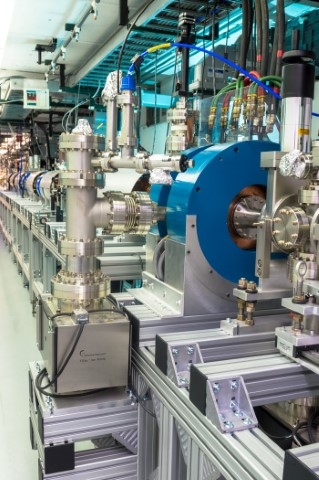
\includegraphics[width=4cm]{../../tex/images/awa_gun}
	\end{minipage}
\end{frame}

\section{Introduction}
\begin{frame}
\frametitle{Argonne Wakefield Accelerator Facility (AWA)}
\Wider[4em]{
	\setlength{\leftmargin}{0.1cm}	
		\begin{itemize}
			\item{Two photocathode guns and linacs}
			\begin{itemize}
				\item{\underline{\textbf{Drive Line}}: $Cs_2Te$ cathode, 6 linac cavities}
				\begin{itemize}
					\item{Charge 0.1-100nC}
					\item{Energy up to 70 MeV}
					
				\end{itemize}
				\item{\underline{\textbf{Witness Line}}: $Mg$ cathode, 1 linac cavity}
				\begin{itemize}
					\item{Charge 0.1-10nC}
					\item{Energy up to 15 MeV}
				\end{itemize}
			\end{itemize}
		\end{itemize}	
		\centering
		\includegraphics[width=0.45\linewidth]{../long_talk/linac}\hspace{0.5em}%
		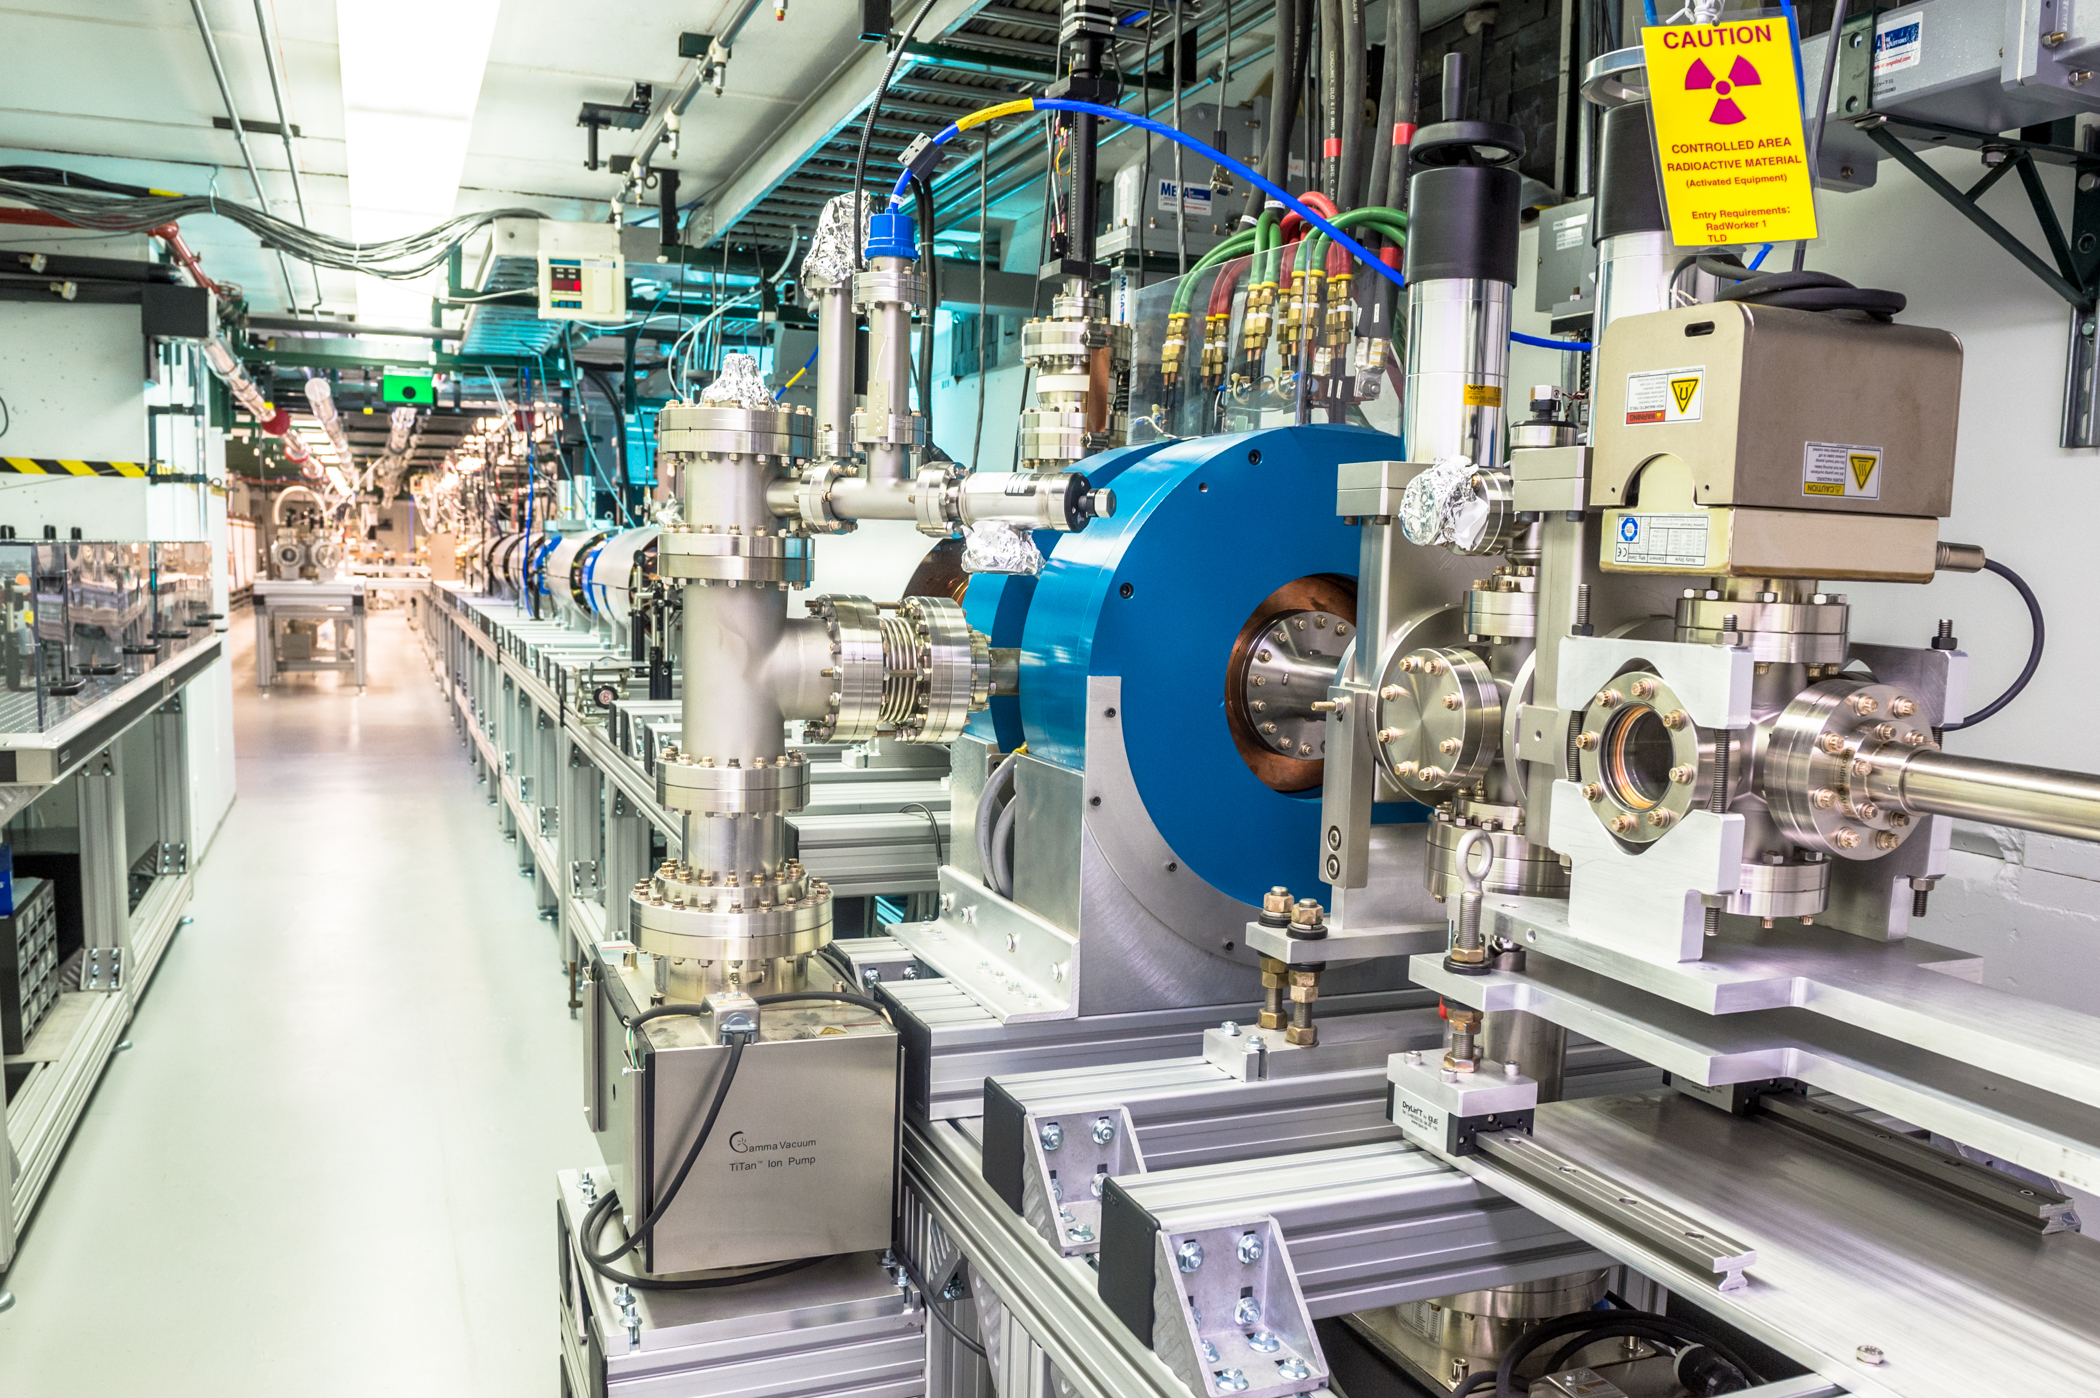
\includegraphics[width=0.45\linewidth]{drive_gun}
}
\end{frame}

\begin{frame}
\frametitle{AWA Facility}
Current experiments include:
\begin{itemize}
	\item{Emittance Exchange (EEX)}
	\item{Electron Radiography Imaging (ERI)}
	\item{Cathode Studies}
	\item Plasma wakefield (very recent)
\end{itemize}
\vspace{0.3cm}
\centering
\includegraphics[height=0.45\textheight]{/home/nicole/Documents/presentations/space_charge_2017/EEX}\hspace{0.5em}%
\includegraphics[height=0.45\textheight]{../long_talk/cathode}
\end{frame}

\begin{frame}
\frametitle{AWA Facility}
Current experiments include:
\begin{itemize}
	\item{Two Beam Acceleration (TBA)}
	\item{Dielectric accelerating and decelerating structure tests}
	\item{Beam line design for TBA = my thesis}
\end{itemize}
\vspace{0.5cm}
\includegraphics[height=0.45\textheight]{/home/nicole/Documents/presentations/space_charge_2017/stage}\hfill\includegraphics[height=0.45\textheight]{/home/nicole/Documents/presentations/space_charge_2017/dielectrics}
\end{frame}
%%%%%%%%%%%%%%%%%%%%%%%%%%%%%%%%%%%%%%%%%%%%%%%%%%%%%%%%%%%%%%%%%%%%%%%%%%%%%%%%%
%%%%%%%%%%%%%%%%%%%%%%%%%%%%%%%%%%%%%%%%%%%%%%%%%%%%%%%%%%%%%%%%%%%%%%%%%%%%%%%%%
%%%%%%%%%%%%%%%%%%%%%%%%%%%%%%%%%%%%%%%%%%%%%%%%%%%%%%%%%%%%%%%%%%%%%%%%%%%%%%%%%
{	\renewcommand{\secimage}{../../tex/images/pets-cst}
\subsection{Two Beam Acceleration (TBA)}
\begin{frame}
	\frametitle{What is Two Beam Acceleration (TBA)?}
	\begin{center}
		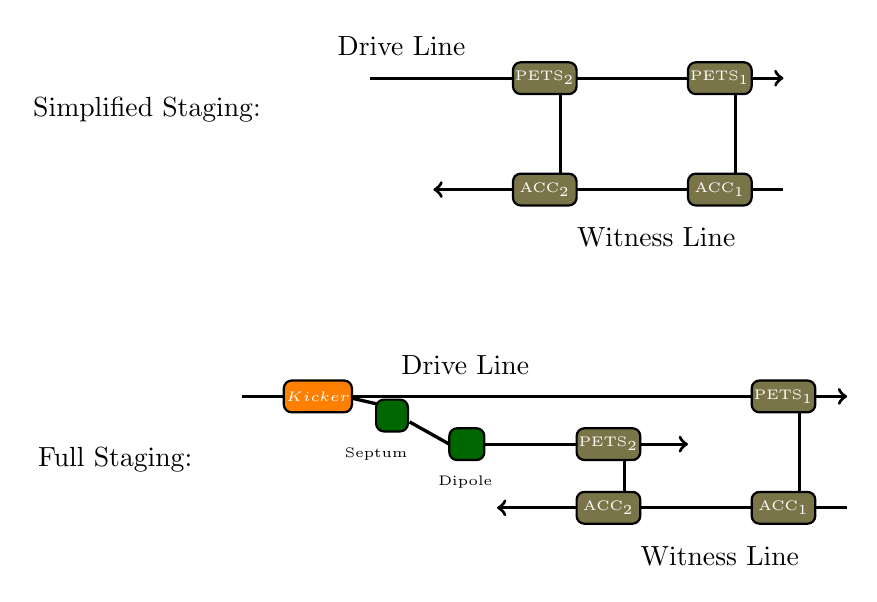
\begin{tikzpicture}[scale=\textwidth/30cm, text=black]
		\def \gunleft {-1.0}
\def \gunright {0.3}
\def \loneright {1.0}
\def \ltworight {2.0}
\def \lthreeright {3.0}
\def \lfourright {4.0}
\def \lfiveright {5.0}
\def \lsixright {6.0}
\def \quadone {7.3}
\def \quadfour{16}

%Full Staging
\draw[very thick, ->] (8,1) -- (27,1);

%Line between kicker and septum
\node[] at (15,2) {Drive Line};
\node[] at (23,-4) {Witness Line};
\draw[very thick] (\lsixright+5.2,1.0) -- (12.5,0.7);

%Kicker 
\draw[fill=orange,  thick, rounded corners =0.1cm] (\lsixright+3.3,0.5)rectangle ({\lsixright+0.84+4.6},1.5) node[pos=.5, white] {\tiny $Kicker$};
%Septum
\node[] at (12.2,-0.8) {\tiny Septum};
\draw[fill=black!60!green,  thick, rounded corners =0.1cm] (12.2,0.9)rectangle ({13.2},-0.1) node[pos=.5, white] {};
%Line between kicker and septum
\draw[very thick] (13.25,0.2) -- (14.5,-0.5);
%Dipole
\node[] at (15,-1.7) {\tiny Dipole};
\draw[fill=black!60!green, thick, rounded corners =0.1cm] (14.5,0.0)rectangle ({15.6},-1.0) node[pos=.5, white] {};
%Line between dipole and quads
\draw[very thick, ->] (15.6,-0.5) -- (22,-0.5);
%Witness
\draw[very thick, <-] (16,-2.5) -- (27,-2.5);
%Waveguide
\draw[very thick] (20,-0.5) -- (20,-3);
%Waveguide
\draw[very thick] (25.5,1.5) -- (25.5,-3);
%PETS2
\draw[fill=black!60!yellow,  thick, rounded corners =0.1cm] (18.5,0.0)rectangle (20.5,-1) node[pos=.5, white] {\tiny$\text{PETS}_2$};
%PETS1
\draw[fill=black!60!yellow,  thick, rounded corners =0.1cm] (24,1.5)rectangle (26,0.5) node[pos=.5, white] {\tiny$\text{PETS}_1$};
%ACC2
\draw[fill=black!60!yellow,  thick, rounded corners =0.1cm] (18.5,-2)rectangle (20.5,-3) node[pos=.5, white] {\tiny$\text{ACC}_2$};
%ACC1
\draw[fill=black!60!yellow,  thick, rounded corners =0.1cm] (24,-2)rectangle (26,-3) node[pos=.5, white] {\tiny$\text{ACC}_1$};



%Simplified Staging



\draw[very thick, ->] (12,11) -- (25,11);

%Line between kicker and septum
\node[] at (13,12) {Drive Line};
\node[] at (21,6) {Witness Line};

%Witness
\draw[very thick, <-] (14,10-2.5) -- (25,10-2.5);
%Waveguide
\draw[very thick] (18,11.5) -- (18,7);
%Waveguide
\draw[very thick] (23.5,11.5) -- (23.5,10-3);
%PETS2
\draw[fill=black!60!yellow,  thick, rounded corners =0.1cm] (16.5,11.5)rectangle (18.5,10.5) node[pos=.5, white] {\tiny$\text{PETS}_2$};
%PETS1
\draw[fill=black!60!yellow,  thick, rounded corners =0.1cm] (22,11.5)rectangle (24,10.5) node[pos=.5, white] {\tiny$\text{PETS}_1$};
%ACC2
\draw[fill=black!60!yellow,  thick, rounded corners =0.1cm] (16.5,8)rectangle (18.5,7) node[pos=.5, white] {\tiny$\text{ACC}_2$};
%ACC1
\draw[fill=black!60!yellow,  thick, rounded corners =0.1cm] (22,8)rectangle (24,7) node[pos=.5, white] {\tiny$\text{ACC}_1$};








		\node[fill=white, inner sep=2pt] (txt2) at (5,10) {Simplified Staging:};
		\node[fill=white, inner sep=2pt] (txt2) at (4,-1) {Full Staging:};
		\end{tikzpicture}
	\end{center}
\end{frame}

\begin{frame}
\frametitle{Power Extraction and Transfer Structure (PETS)}
\begin{itemize}
	\item Form factor and bunch length are related. 
	\item Charge and bunch length drive power extraction
\end{itemize}
\begin{minipage}{0.45\textwidth}
	\begin{flalign*}
	\alpha & = \frac{\omega}{2 Q_{cavity} v_g}  
	\end{flalign*}
	\begin{flalign*}
	P_t & = \frac{\omega \textcolor{red}{Q^2} }{4 v_g} \frac{R}{ Q_{cavity} } \frac{1-e^{-\alpha L}}{\alpha} \textcolor{red}{\phi^2}
	\end{flalign*}
\end{minipage}\hfill
\begin{minipage}{0.5\textwidth}
	\centering
	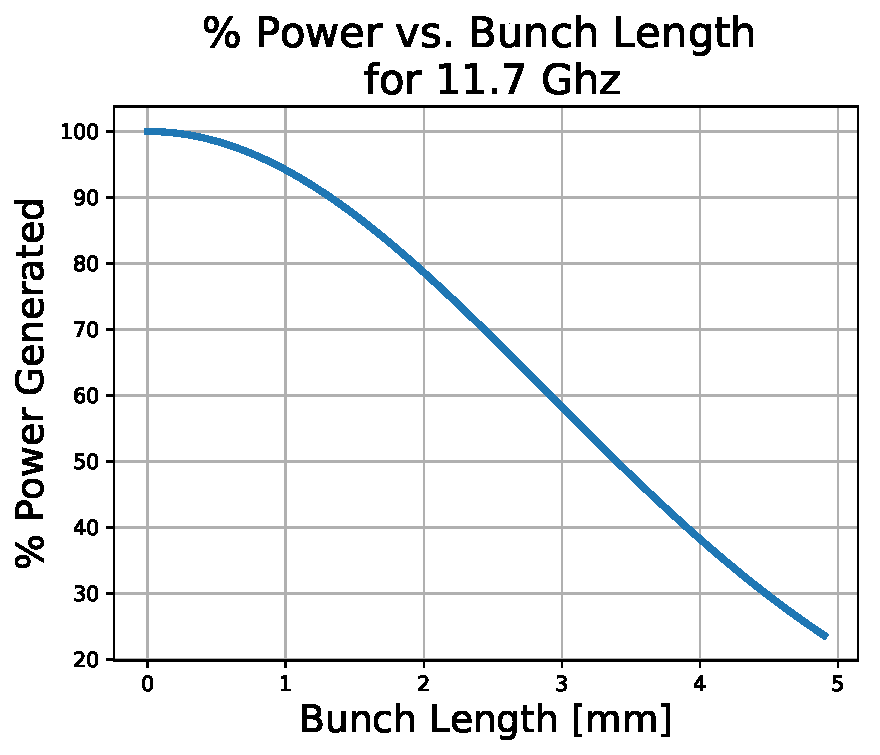
\includegraphics[height=\textwidth]{../../tex/images/formfactorsqrd}
\end{minipage}
\end{frame}

\begin{frame}
\frametitle{Simplified Staging Details}
\begin{itemize}
	\item Metallic structures; 17.6 mm (PETS) or 6 mm (ACC) aperture
	\item Two stage, average 70 MeV/m 
	\item 4.9 MeV energy gain in past tests 
	\item Single stage test result in higher gradients (150 MeV/m)
\end{itemize}
\vspace{0.5em}
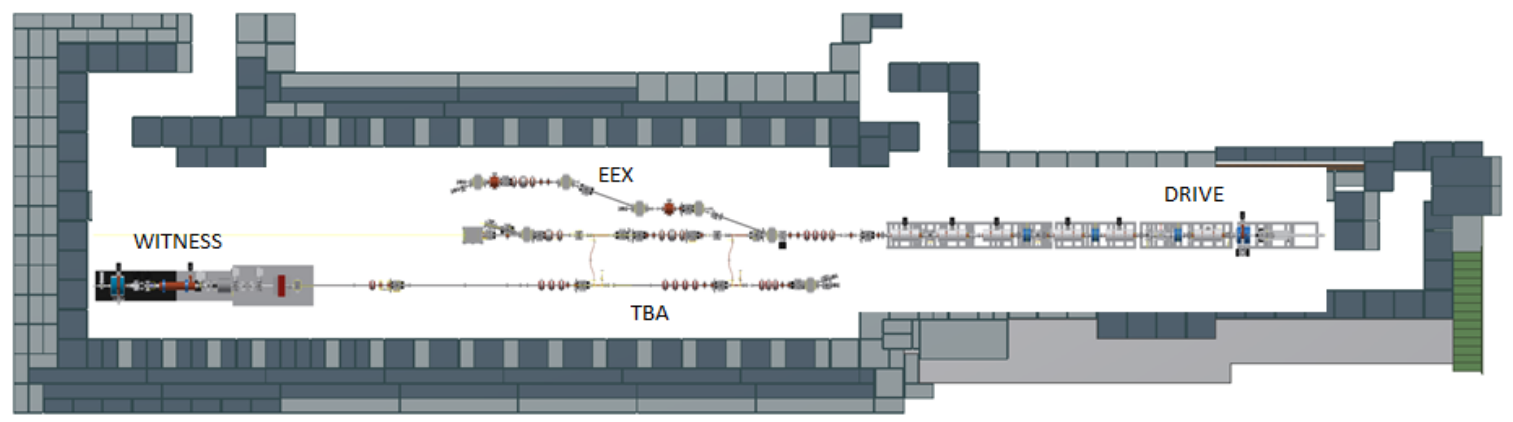
\includegraphics[width=\linewidth]{../../tex/images/bunker}
\tiny{*Drawing courtesy of S. Doran}
\end{frame}

\begin{frame}
\Wider[5em]{
	\frametitle{Full Staging}
	\begin{center}
		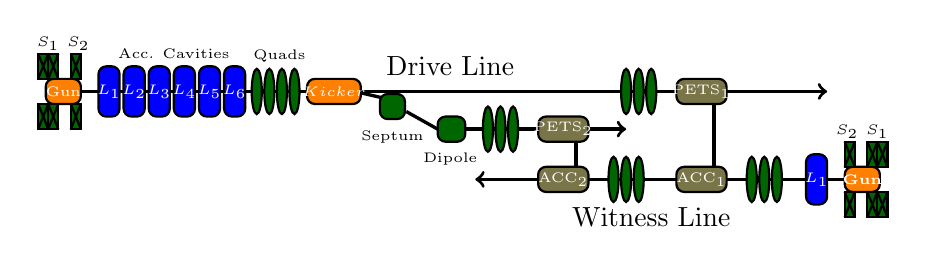
\begin{tikzpicture}[scale=\textwidth/38cm, text=black]
		%\begin{tikzpicture}[scale=0.5, text=black]
		\def \gunleft {-1.0}
\def \gunright {0.3}
\def \loneright {1.0}
\def \ltworight {2.0}
\def \lthreeright {3.0}
\def \lfourright {4.0}
\def \lfiveright {5.0}
\def \lsixright {6.0}
\def \quadone {7.3}
\def \quadfour{16}

\draw[very thick, ->] (0.0,1) -- (30,1);

\draw[fill=orange, thick, rounded corners =0.1cm] (\gunleft-0.1,0.5)rectangle (\gunright,1.5) node[pos=.5, white] {\small{\tiny{Gun}}} ;
%Straight through

%S1
\node[] at (-1,2.9) {\tiny $S_1$};
\draw[thick, fill=black!60!green] (-1.4,-0.5)rectangle  (-1.0,0.5) node[pos=.5, white] {} ;
\draw[black,  thick] (-1.4,-0.5) -- (-1.0,0.5);
\draw[black,  thick] (-1.4,0.5) -- (-1.0,-0.5);
\draw[ thick, fill=black!60!green] (-1.4,1.5)rectangle  (-1.0,2.5) node[pos=.5, white] {} ;
\draw[black,  thick] (-1.4,1.5) -- (-1.0,2.5);
\draw[black,  thick] (-1.4,2.5) -- (-1.0,1.5);

\draw[ thick, fill=black!60!green] (-1.0,-0.5)rectangle  (-0.6,0.5) node[pos=.5, white] {} ;
\draw[black,  thick] (-1.0,-0.5) -- (-0.6,0.5);
\draw[black,  thick] (-1.0,0.5) -- (-0.6,-0.5);
\draw[ thick, fill=black!60!green] (-1.0,1.5)rectangle  (-0.6,2.5) node[pos=.5, white] {} ;
\draw[black,  thick] (-1.0,1.5) -- (-0.6,2.5);
\draw[black,  thick] (-1.0,2.5) -- (-0.6,1.5);

%S2
\node[] at (0.2,2.9) {\tiny $S_2$};
\draw[ thick, fill=black!60!green] (-0.1,-0.5) rectangle  (0.3,0.5) node[pos=.5, white] {};
\draw[black,  thick] (-0.1,-0.5) -- (0.3,0.5);
\draw[black,  thick] (-0.1,0.5) -- (0.3,-0.5);
\draw[ thick, fill=black!60!green] (-0.1,1.5) rectangle  (0.3,2.5) node[pos=.5, white] {};
\draw[black,  thick] (-0.1,1.5) -- (0.3,2.5);
\draw[black,  thick] (-0.1,2.5) -- (0.3,1.5);
%Linac drawings 
\node[] at (4,2.5) {\tiny Acc. Cavities};
\draw[fill=blue,  thick, rounded corners =0.1cm] (\loneright,0)rectangle  ({\loneright+0.84},2) node[pos=.5, white] {\tiny $L_1$} ;
\draw[fill=blue,  thick, rounded corners =0.1cm] (\ltworight,0)rectangle  ({\ltworight+0.84},2) node[pos=.5, white] {\tiny $L_2$};
\draw[fill=blue,  thick, rounded corners =0.1cm] (\lthreeright,0)rectangle ({\lthreeright+0.84},2) node[pos=.5, white] {\tiny $L_3$};
\draw[fill=blue,  thick, rounded corners =0.1cm] (\lfourright,0)rectangle ({\lfourright+0.84},2) node[pos=.5, white] {\tiny $L_4$};
\draw[fill=blue,  thick, rounded corners =0.1cm] (\lfiveright,0)rectangle ({\lfiveright+0.84},2) node[pos=.5, white] {\tiny $L_5$};
\draw[fill=blue,  thick, rounded corners =0.1cm] (\lsixright,0)rectangle ({\lsixright+0.84},2) node[pos=.5, white] {\tiny $L_6$};

%current optimization point
%\node[draw, fill=yellow, star, star points=5, star point ratio=0.6, minimum size=0.1cm]
%at (12.5,1.0) {$z_1$};


%Quad drawings
\node[] at (8.2,2.4) {\tiny{Quads}};
\draw[fill=black!60!green,  thick] (\quadone, 1.0) ellipse (0.2cm and 0.9cm);
\draw[fill=black!60!green,  thick] (\quadone+0.5, 1.0) ellipse (0.2cm and 0.9cm);
\draw[fill=black!60!green,  thick] (\quadone+1.0, 1.0) ellipse (0.2cm and 0.9cm);
\draw[fill=black!60!green,  thick] (\quadone+1.5, 1.0) ellipse (0.2cm and 0.9cm);

%Line between kicker and septum
\node[] at (15,2) {Drive Line};
\node[] at (23,-4) {Witness Line};
\draw[very thick] (\lsixright+5.2,1.0) -- (12.5,0.7);

%Kicker 
\draw[fill=orange,  thick, rounded corners =0.1cm] (\lsixright+3.3,0.5)rectangle ({\lsixright+0.84+4.6},1.5) node[pos=.5, white] {\tiny $Kicker$};

%Septum
\node[] at (12.7,-0.8) {\tiny Septum};
\draw[fill=black!60!green,  thick, rounded corners =0.1cm] (12.2,0.9)rectangle ({13.2},-0.1) node[pos=.5, white] {};
%\draw[latex-latex] (\gunleft,-5.0) -- (14,-5.0) ;
%\foreach \x in  {0.3, 1.0, 3.5, 5.0, 7.0, 8.5, 10, 12.5} %tick marks
%\draw[shift={(\x,-5.0)},color=black] (0pt,3pt) -- (0pt,-3pt);
%\foreach \x in {0.3, 1.0, 3.5, 5.0, 7.0, 8.5, 10, 12.5}
%\draw[shift={(\x,-5.2)},color=black] (0pt,0pt) node[below] {$\x$};

%Line between kicker and septum
\draw[very thick] (13.25,0.2) -- (14.5,-0.5);

%Dipole
\node[] at (15,-1.7) {\tiny Dipole};
\draw[fill=black!60!green, thick, rounded corners =0.1cm] (14.5,0.0)rectangle ({15.6},-1.0) node[pos=.5, white] {};

%Line between dipole and quads
\draw[very thick, ->] (15.6,-0.5) -- (22,-0.5);
%Second set of quads
\draw[fill=black!60!green,  thick] (\quadfour+0.5, -0.50) ellipse (0.2cm and 0.9cm);
\draw[fill=black!60!green,  thick] (\quadfour+1.0, -0.50) ellipse (0.2cm and 0.9cm);
\draw[fill=black!60!green,  thick] (\quadfour+1.5, -0.50) ellipse (0.2cm and 0.9cm);



\def \quadfive{22}
%Third set of quads
\draw[fill=black!60!green,  thick] (\quadfive, 1.0) ellipse (0.2cm and 0.9cm);
\draw[fill=black!60!green,  thick] (\quadfive+0.5, 1.0) ellipse (0.2cm and 0.9cm);
\draw[fill=black!60!green,  thick] (\quadfive+1.0, 1.0) ellipse (0.2cm and 0.9cm);


%Witness
\draw[very thick, <-] (16,-2.5) -- (31,-2.5);

%Waveguide
\draw[very thick] (20,-0.5) -- (20,-3);
%Waveguide
\draw[very thick] (25.5,1.5) -- (25.5,-3);

%PETS2
\draw[fill=black!60!yellow,  thick, rounded corners =0.1cm] (18.5,0.0)rectangle (20.5,-1) node[pos=.5, white] {\tiny$\text{PETS}_2$};
%PETS1
\draw[fill=black!60!yellow,  thick, rounded corners =0.1cm] (24,1.5)rectangle (26,0.5) node[pos=.5, white] {\tiny$\text{PETS}_1$};

%ACC2
\draw[fill=black!60!yellow,  thick, rounded corners =0.1cm] (18.5,-2)rectangle (20.5,-3) node[pos=.5, white] {\tiny$\text{ACC}_2$};
%ACC1
\draw[fill=black!60!yellow,  thick, rounded corners =0.1cm] (24,-2)rectangle (26,-3) node[pos=.5, white] {\tiny$\text{ACC}_1$};
\def \quadsix{27}
%Third set of quads
\draw[fill=black!60!green,  thick] (\quadsix, -2.5) ellipse (0.2cm and 0.9cm);
\draw[fill=black!60!green,  thick] (\quadsix+0.5, -2.5) ellipse (0.2cm and 0.9cm);
\draw[fill=black!60!green,  thick] (\quadsix+1.0, -2.5) ellipse (0.2cm and 0.9cm);
\def \quadseven{21.5}
%Third set of quads
\draw[fill=black!60!green,  thick] (\quadseven, -2.5) ellipse (0.2cm and 0.9cm);
\draw[fill=black!60!green,  thick] (\quadseven+0.5, -2.5) ellipse (0.2cm and 0.9cm);
\draw[fill=black!60!green,  thick] (\quadseven+1.0, -2.5) ellipse (0.2cm and 0.9cm);

\begin{scope}[yscale=1,xscale=-1, yshift=-3.5cm, xshift=-31cm]
	\draw[fill=orange, thick, rounded corners =0.1cm] (\gunleft-0.1,0.5)rectangle (\gunright,1.5) node[pos=.5, white] {\textbf{\tiny Gun}} ;
	
	%S1
	\node[] at (-1,2.9) {\tiny$S_1$};
	\draw[thick, fill=black!60!green] (-1.4,-0.5)rectangle  (-1.0,0.5) node[pos=.5, white] {} ;
	\draw[black,  thick] (-1.4,-0.5) -- (-1.0,0.5);
	\draw[black,  thick] (-1.4,0.5) -- (-1.0,-0.5);
	\draw[ thick, fill=black!60!green] (-1.4,1.5)rectangle  (-1.0,2.5) node[pos=.5, white] {} ;
	\draw[black,  thick] (-1.4,1.5) -- (-1.0,2.5);
	\draw[black,  thick] (-1.4,2.5) -- (-1.0,1.5);
	
	\draw[ thick, fill=black!60!green] (-1.0,-0.5)rectangle  (-0.6,0.5) node[pos=.5, white] {} ;
	\draw[black,  thick] (-1.0,-0.5) -- (-0.6,0.5);
	\draw[black,  thick] (-1.0,0.5) -- (-0.6,-0.5);
	\draw[ thick, fill=black!60!green] (-1.0,1.5)rectangle  (-0.6,2.5) node[pos=.5, white] {} ;
	\draw[black,  thick] (-1.0,1.5) -- (-0.6,2.5);
	\draw[black,  thick] (-1.0,2.5) -- (-0.6,1.5);
	
	%S2
	\node[] at (0.2,2.9) {\tiny$S_2$};
	\draw[ thick, fill=black!60!green] (-0.1,-0.5) rectangle  (0.3,0.5) node[pos=.5, white] {};
	\draw[black,  thick] (-0.1,-0.5) -- (0.3,0.5);
	\draw[black,  thick] (-0.1,0.5) -- (0.3,-0.5);
	\draw[ thick, fill=black!60!green] (-0.1,1.5) rectangle  (0.3,2.5) node[pos=.5, white] {};
	\draw[black,  thick] (-0.1,1.5) -- (0.3,2.5);
	\draw[black,  thick] (-0.1,2.5) -- (0.3,1.5);
	%Linac drawings 
	%\node[] at (4,2.5) {Accelerating Cavities};
	\draw[fill=blue,  thick, rounded corners =0.1cm] (\loneright,0)rectangle  ({\loneright+0.84},2) node[pos=.5, white] {\tiny$L_1$} ;
	
\end{scope}



		\end{tikzpicture}
	\end{center}
}	
\begin{itemize}
	\item Maintain modular design 
	\item Maximize power in each stage
	\item Plug and play various structures	
\end{itemize}
\end{frame}
}
%%%%%%%%%%%%%%%%%%%%%%%%%%%%%%%%%%%%%%%%%%%%%%%%%%%%%%%%%%%%%%%%%%%%%%%%%%%%%%%%%
%%%%%%%%%%%%%%%%%%%%%%%%%%%%%%%%%%%%%%%%%%%%%%%%%%%%%%%%%%%%%%%%%%%%%%%%%%%%%%%%%
%%%%%%%%%%%%%%%%%%%%%%%%%%%%%%%%%%%%%%%%%%%%%%%%%%%%%%%%%%%%%%%%%%%%%%%%%%%%%%%%%
{
	\renewcommand{\secimage}{../../tex/images/YAG1_40nC}
\section{Simulations}
\begin{frame}
\frametitle{Code and Resources: }
OPAL, Python (Main Codes of Choice)
\begin{minipage}{0.5\textwidth}
	\begin{itemize}
		\item Free
		\item Parallel 
		\item Open Source
		\item 3D space charge (40 nC)
	\end{itemize}	
\end{minipage}
\begin{minipage}{0.4\textwidth}
	\vspace{0.5em}
	HPC Resources Used:
	\begin{itemize}
		\item Blues, ANL
		\item Bebop, ANL
		\item Theta, ANL
		\item Merlin, PSI (briefly)
	\end{itemize}
\end{minipage}
\begin{center}
\vspace{0.5em}
\includegraphics[height=0.4\textheight]{../comp_talk/bebop} \hspace{1em} \includegraphics[height=0.4\textheight]{../comp_talk/theta}
\end{center}
\end{frame}

\begin{frame}
\frametitle{Benchmark: ASTRA, GPT, OPAL-T}
\vspace{2em}
\Wider[4em]{
\begin{minipage}{0.75\textwidth}
	\begin{itemize}
		\item{Motivated by code features and my inexperience}
		\item{Used RF and solenoid maps from AWA photocathode gun}
		\begin{itemize}
			\item 2D SUPERFISH/POISSON
		\end{itemize}
		\item{Used PITZ operating conditions as input parameters}
		\item{Spoiler: No major differences found at 1 nC}
		\begin{itemize}
			\item However, a lot of work to match input parameters
		\end{itemize}
	\end{itemize}
\end{minipage}
\begin{minipage}{0.2\textwidth}
	\def \gunleft {-1.0}
	\def \gunright {0.3}
	\def \loneright {1.0}
	\def \ltworight {3.5}
	\def \lthreeright {5.0}
	\def \lfourright {7.0}
	\def \lfiveright {8.5}
	\def \lsixright {10}
	\begin{center}
		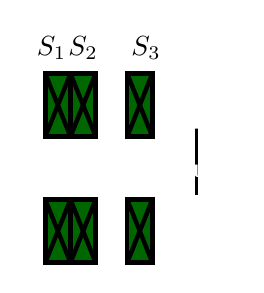
\begin{tikzpicture}[scale=0.8]
		%Gun drawings
		\draw[fill=orange, very thick, rounded corners =0.1cm] (\gunleft,0.5)rectangle (\gunright,1.5) node[pos=.5, white] {\textbf{Gun}} ;
		%S1
		\node[] at (-1.3,2.9) {$S_1$};
		\draw[ultra thick, fill=black!60!green] (-1.4,-0.5)rectangle  (-1.0,0.5) node[pos=.5, white] {} ;
		\draw[black, ultra thick] (-1.4,-0.5) -- (-1.0,0.5);
		\draw[black, ultra thick] (-1.4,0.5) -- (-1.0,-0.5);
		\draw[ultra thick, fill=black!60!green] (-1.4,1.5)rectangle  (-1.0,2.5) node[pos=.5, white] {} ;
		\draw[black, ultra thick] (-1.4,1.5) -- (-1.0,2.5);
		\draw[black, ultra thick] (-1.4,2.5) -- (-1.0,1.5);
		%S2
		\node[] at (-0.8,2.9) {$S_2$};
		\draw[ultra thick, fill=black!60!green] (-1.0,-0.5)rectangle  (-0.6,0.5) node[pos=.5, white] {} ;
		\draw[black, ultra thick] (-1.0,-0.5) -- (-0.6,0.5);
		\draw[black, ultra thick] (-1.0,0.5) -- (-0.6,-0.5);
		\draw[ultra thick, fill=black!60!green] (-1.0,1.5)rectangle  (-0.6,2.5) node[pos=.5, white] {} ;
		\draw[black, ultra thick] (-1.0,1.5) -- (-0.6,2.5);
		\draw[black, ultra thick] (-1.0,2.5) -- (-0.6,1.5);
		%S3
		\node[] at (0.2,2.9) {$S_3$};
		\draw[ultra thick, fill=black!60!green] (-0.1,-0.5) rectangle  (0.3,0.5) node[pos=.5, white] {};
		\draw[black, ultra thick] (-0.1,-0.5) -- (0.3,0.5);
		\draw[black, ultra thick] (-0.1,0.5) -- (0.3,-0.5);
		\draw[ultra thick, fill=black!60!green] (-0.1,1.5) rectangle  (0.3,2.5) node[pos=.5, white] {};
		\draw[black, ultra thick] (-0.1,1.5) -- (0.3,2.5);
		\draw[black, ultra thick] (-0.1,2.5) -- (0.3,1.5);
		\end{tikzpicture}
	\end{center}
\end{minipage}
}
\end{frame}

\begin{frame}
\frametitle{Benchmark Results}
\Wider[4em]{
All codes matched within $5\%$. \\
Below precision of diagnostics at AWA.\\  
\vskip12pt
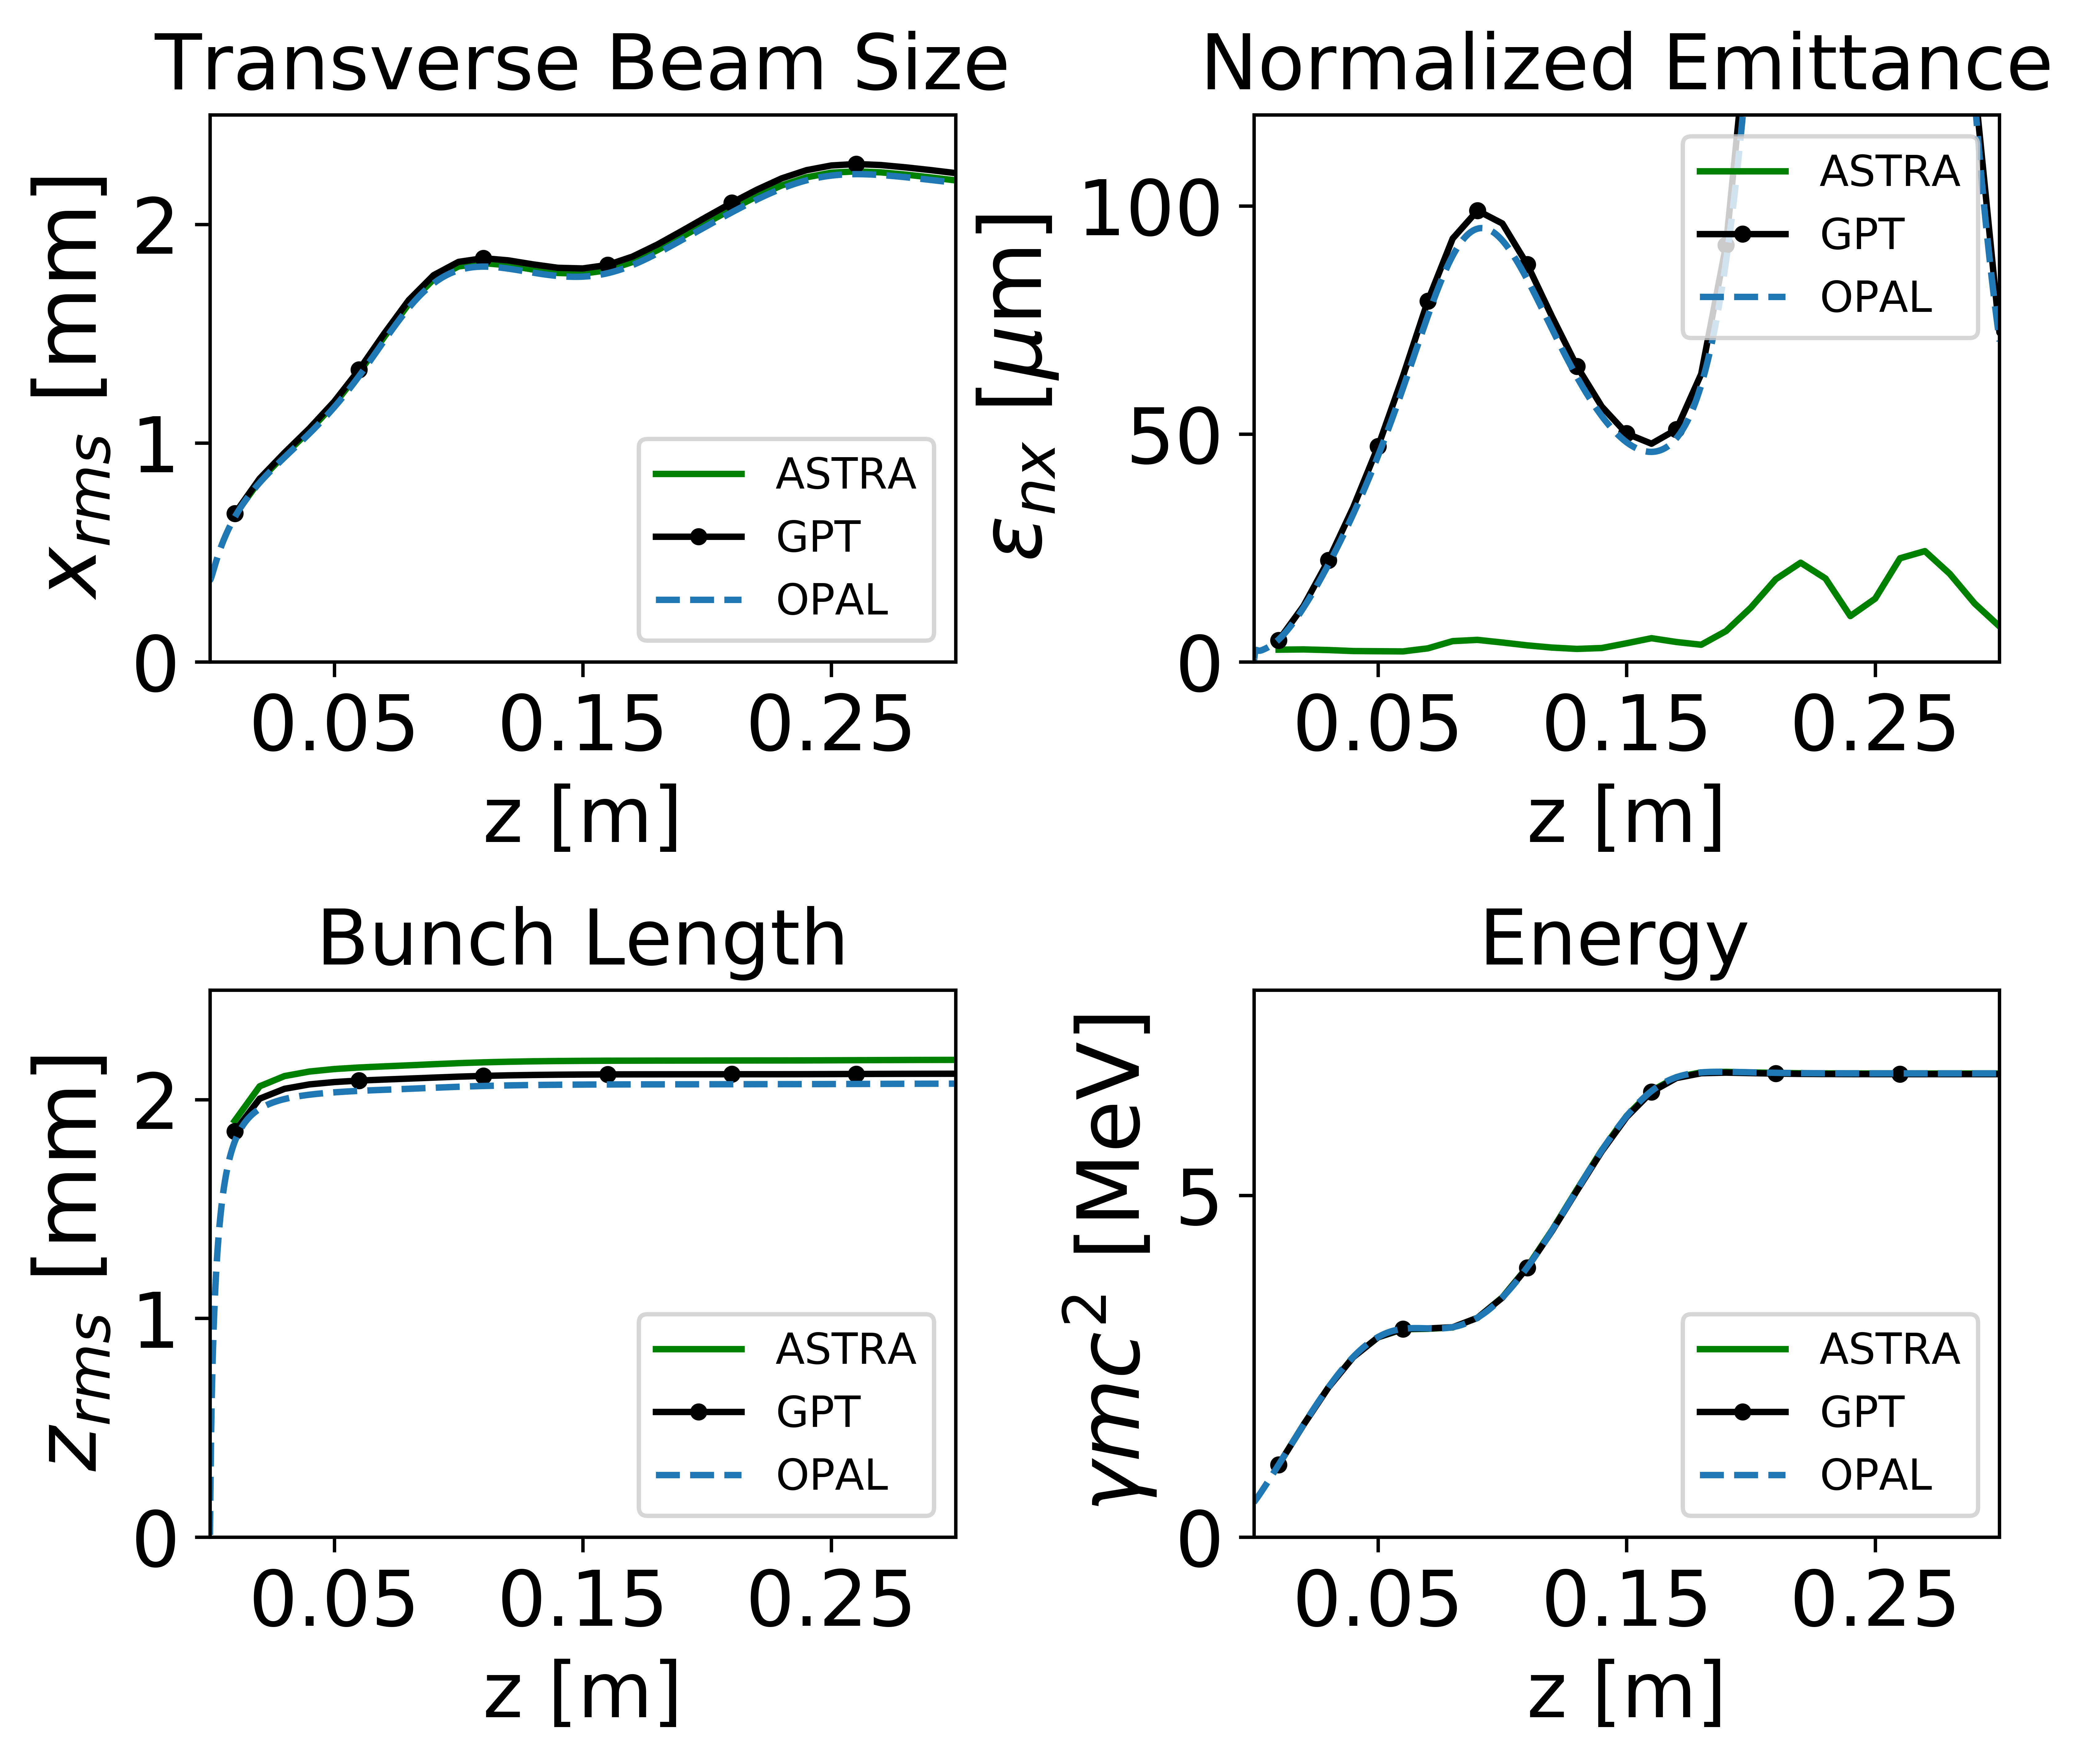
\includegraphics[width=0.49\linewidth]{../../tex/images/benchmark_gun}\hfill 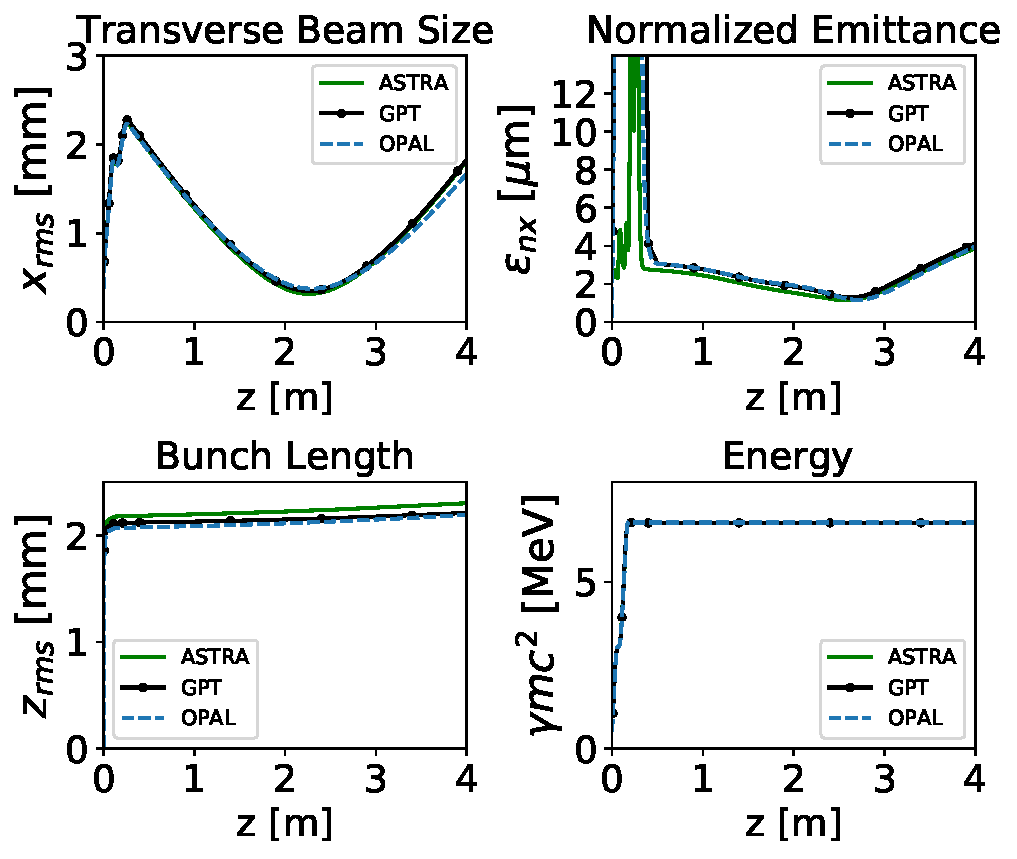
\includegraphics[width=0.49\linewidth]{../../tex/images/benchmark_5m}
}
\end{frame}

\begin{frame}
	\frametitle{Optimization}
	\begin{itemize}
		\item Needed to improve transmission of 40 nC trains
		\item Judge trade off between beam parameters
		\item Usually compare emittance, beam size, and/or bunch length
	\end{itemize}
\begin{minipage}{0.35\linewidth}
	Some jargon:
	\begin{itemize}
		\item Objectives
		\item Design Variables
		\item Pareto Front
	\end{itemize}
\end{minipage}
\begin{minipage}{0.6\linewidth}
	\includegraphics[width=\linewidth]{/home/nicole/Documents/presentations/ipac2018/opt-ipac18/paper-pareto-ex-vs-rmss}
\end{minipage}
\end{frame}

\begin{frame}
\frametitle{Optimization (Linac only)}
\Wider[4em]{
\begin{minipage}{0.6\textwidth}
	\begin{itemize}
		\item{Determine what emittance and bunch length we can expect from the linac}
		\begin{itemize}
			\item After $L_6$: $z_1=12.51$ m
		\end{itemize}
		\item{Used algorithm BOBYQA from NLopt}
		\item{Varied 10 parameters:}
	\end{itemize}
\end{minipage}%
\begin{minipage}{0.4\textwidth}
	\def \gunleft {-1.0}
	\def \gunright {0.3}
	\def \loneright {1.0}
	\def \ltworight {2.0}
	\def \lthreeright {3.0}
	\def \lfourright {4.0}
	\def \lfiveright {5.0}
	\def \lsixright {6.0}
	\centering
	\begin{center}
		\begin{tikzpicture}[scale=0.55]%,use optics
		%Gun drawings
		\draw[fill=orange, very thick, rounded corners =0.1cm] (\gunleft-0.2,0.5)rectangle (\gunright,1.5) node[pos=.5, white] {\textbf{Gun}} ;	
		%S1
		\node[] at (-1.5,2.9) {$S_1$};
		\draw[ultra thick, fill=black!60!green] (-1.4,-0.5)rectangle  (-1.0,0.5) node[pos=.5, white] {} ;
		\draw[black, ultra thick] (-1.4,-0.5) -- (-1.0,0.5);
		\draw[black, ultra thick] (-1.4,0.5) -- (-1.0,-0.5);
		\draw[ultra thick, fill=black!60!green] (-1.4,1.5)rectangle  (-1.0,2.5) node[pos=.5, white] {} ;
		\draw[black, ultra thick] (-1.4,1.5) -- (-1.0,2.5);
		\draw[black, ultra thick] (-1.4,2.5) -- (-1.0,1.5);
		%S2
		\node[] at (-0.8,2.9) {$S_2$};
		\draw[ultra thick, fill=black!60!green] (-1.0,-0.5)rectangle  (-0.6,0.5) node[pos=.5, white] {} ;
		\draw[black, ultra thick] (-1.0,-0.5) -- (-0.6,0.5);
		\draw[black, ultra thick] (-1.0,0.5) -- (-0.6,-0.5);
		\draw[ultra thick, fill=black!60!green] (-1.0,1.5)rectangle  (-0.6,2.5) node[pos=.5, white] {} ;
		\draw[black, ultra thick] (-1.0,1.5) -- (-0.6,2.5);
		\draw[black, ultra thick] (-1.0,2.5) -- (-0.6,1.5);		
		%S3
		\node[] at (0.2,2.9) {$S_3$};
		\draw[ultra thick, fill=black!60!green] (-0.1,-0.5) rectangle  (0.3,0.5) node[pos=.5, white] {};
		\draw[black, ultra thick] (-0.1,-0.5) -- (0.3,0.5);
		\draw[black, ultra thick] (-0.1,0.5) -- (0.3,-0.5);
		\draw[ultra thick, fill=black!60!green] (-0.1,1.5) rectangle  (0.3,2.5) node[pos=.5, white] {};
		\draw[black, ultra thick] (-0.1,1.5) -- (0.3,2.5);
		\draw[black, ultra thick] (-0.1,2.5) -- (0.3,1.5);
		%Linac drawings 
		\draw[fill=blue, ultra thick, rounded corners =0.1cm] (\loneright,0)rectangle  ({\loneright+0.84},2) node[pos=.5, white] {$L_1$} ;
		\draw[fill=blue, ultra thick, rounded corners =0.1cm] (\ltworight,0)rectangle  ({\ltworight+0.84},2) node[pos=.5, white] {$L_2$};
		\draw[fill=blue, ultra thick, rounded corners =0.1cm] (\lthreeright,0)rectangle ({\lthreeright+0.84},2) node[pos=.5, white] {$L_3$};
		\draw[fill=blue, ultra thick, rounded corners =0.1cm] (\lfourright,0)rectangle ({\lfourright+0.84},2) node[pos=.5, white] {$L_4$};
		\draw[fill=blue, ultra thick, rounded corners =0.1cm] (\lfiveright,0)rectangle ({\lfiveright+0.84},2) node[pos=.5, white] {$L_5$};
		\draw[fill=blue, ultra thick, rounded corners =0.1cm] (\lsixright,0)rectangle ({\lsixright+0.84},2) node[pos=.5, white] {$L_6$};
		\end{tikzpicture}
	\end{center}
\end{minipage}%
\begin{center}
	\setcounter{mpfootnote}{\value{footnote}}%
	\renewcommand{\thempfootnote}{\arabic{mpfootnote}}%	
	\begin{tabular}{ l *{3}{c}}
		%\toprule
		\textbf{Variable} & \textbf{Range} & \textbf{Unit} \\
		\midrule
		Solenoid Strength & $ 0 \le S_3 \le 440$  & amps \\
		Phase of Gun & $-60 \le \phi_g \le 60$  & degrees \\
		Laser Radius  & $0.1 \le R \le 30$  & mm \\
		Laser FWHM  & $2 \le T \le $10  & ps \\
		Cavity Phase & $-20 \le \phi_L \le 20$\footnote[1]{$\phi_L=[\phi_{L_1},\ldots,\phi_{L_6}]$} & degrees
		%\bottomrule    
	\end{tabular}
\end{center}
}
\end{frame}

\subsection{Model Based and Genetic Algorithms}
\begin{frame}
\frametitle{Linac Optimization (scalarization)}
\begin{itemize}
\item{1,000 point sample was done}
\item{132 simulations completed w/o error}
\item{Scaled and shifted raw values to remove unit dependence}
\end{itemize}
\begin{align*}
\bar{\epsilon}_x (v,z_1) = \frac{ \epsilon_x (v,z_1) - \epsilon_{\min} } { \epsilon_{\max} - \epsilon_{\min} }
\end{align*}
\begin{itemize}
\item{Used 11 weights from 0-1}
\item{Solved 11 optimization problems $f(v,w)$ using BOBYQA}
\end{itemize}
\begin{gather*}
w\in\left\{ 0, \,0.1, \,0.2, \ldots, 1 \right\}\\ \\
f(v,w) = w \,\bar{\epsilon}_x(v,z_1) + (1-w)\, \bar{\sigma}_z(v,z_1)
\end{gather*}
\end{frame}

\begin{frame}
\frametitle{BOBYQA Results}
\vspace{2em}
\Wider[4em]{
\begin{minipage}{0.5\textwidth}
	Convergence of function minimum vs. \\
	number of evaluations per weights.
	\centering
	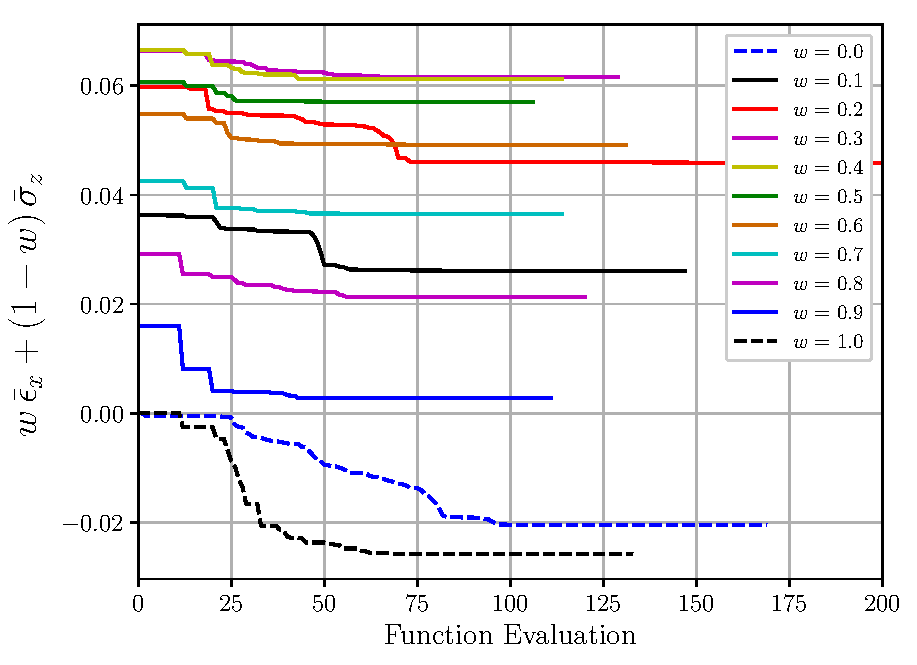
\includegraphics[width=\textwidth]{../../tex/images/THPAB155f2}
\end{minipage}
\begin{minipage}{0.49\textwidth}
	\centering
	Trade off between emittance and bunch length
	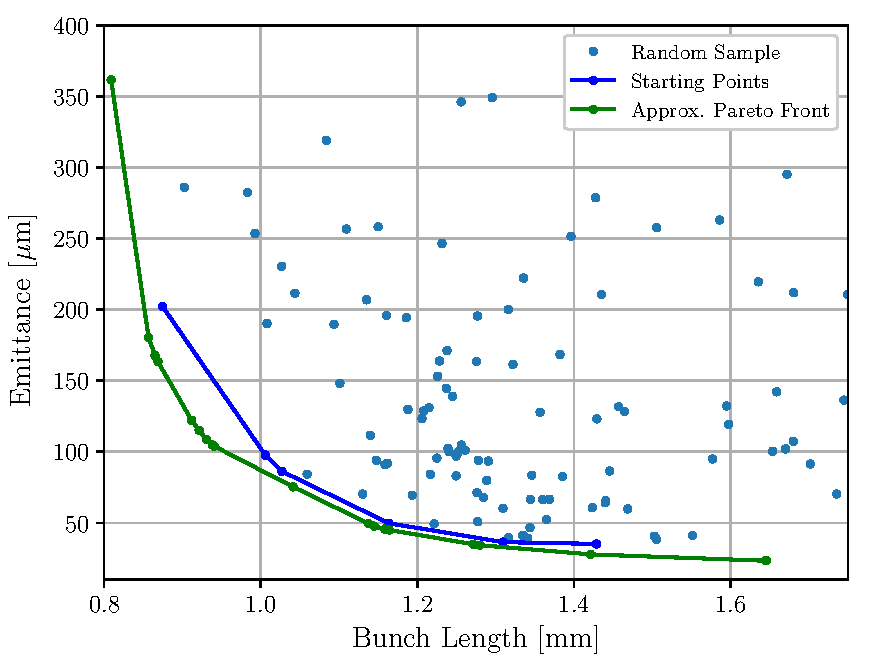
\includegraphics[width=\textwidth]{../../tex/images/THPAB155f1}%
\end{minipage}
}
\end{frame}

\begin{frame}
\frametitle{Validation of Model Based Results}
\vspace{-0.5em}
\centering
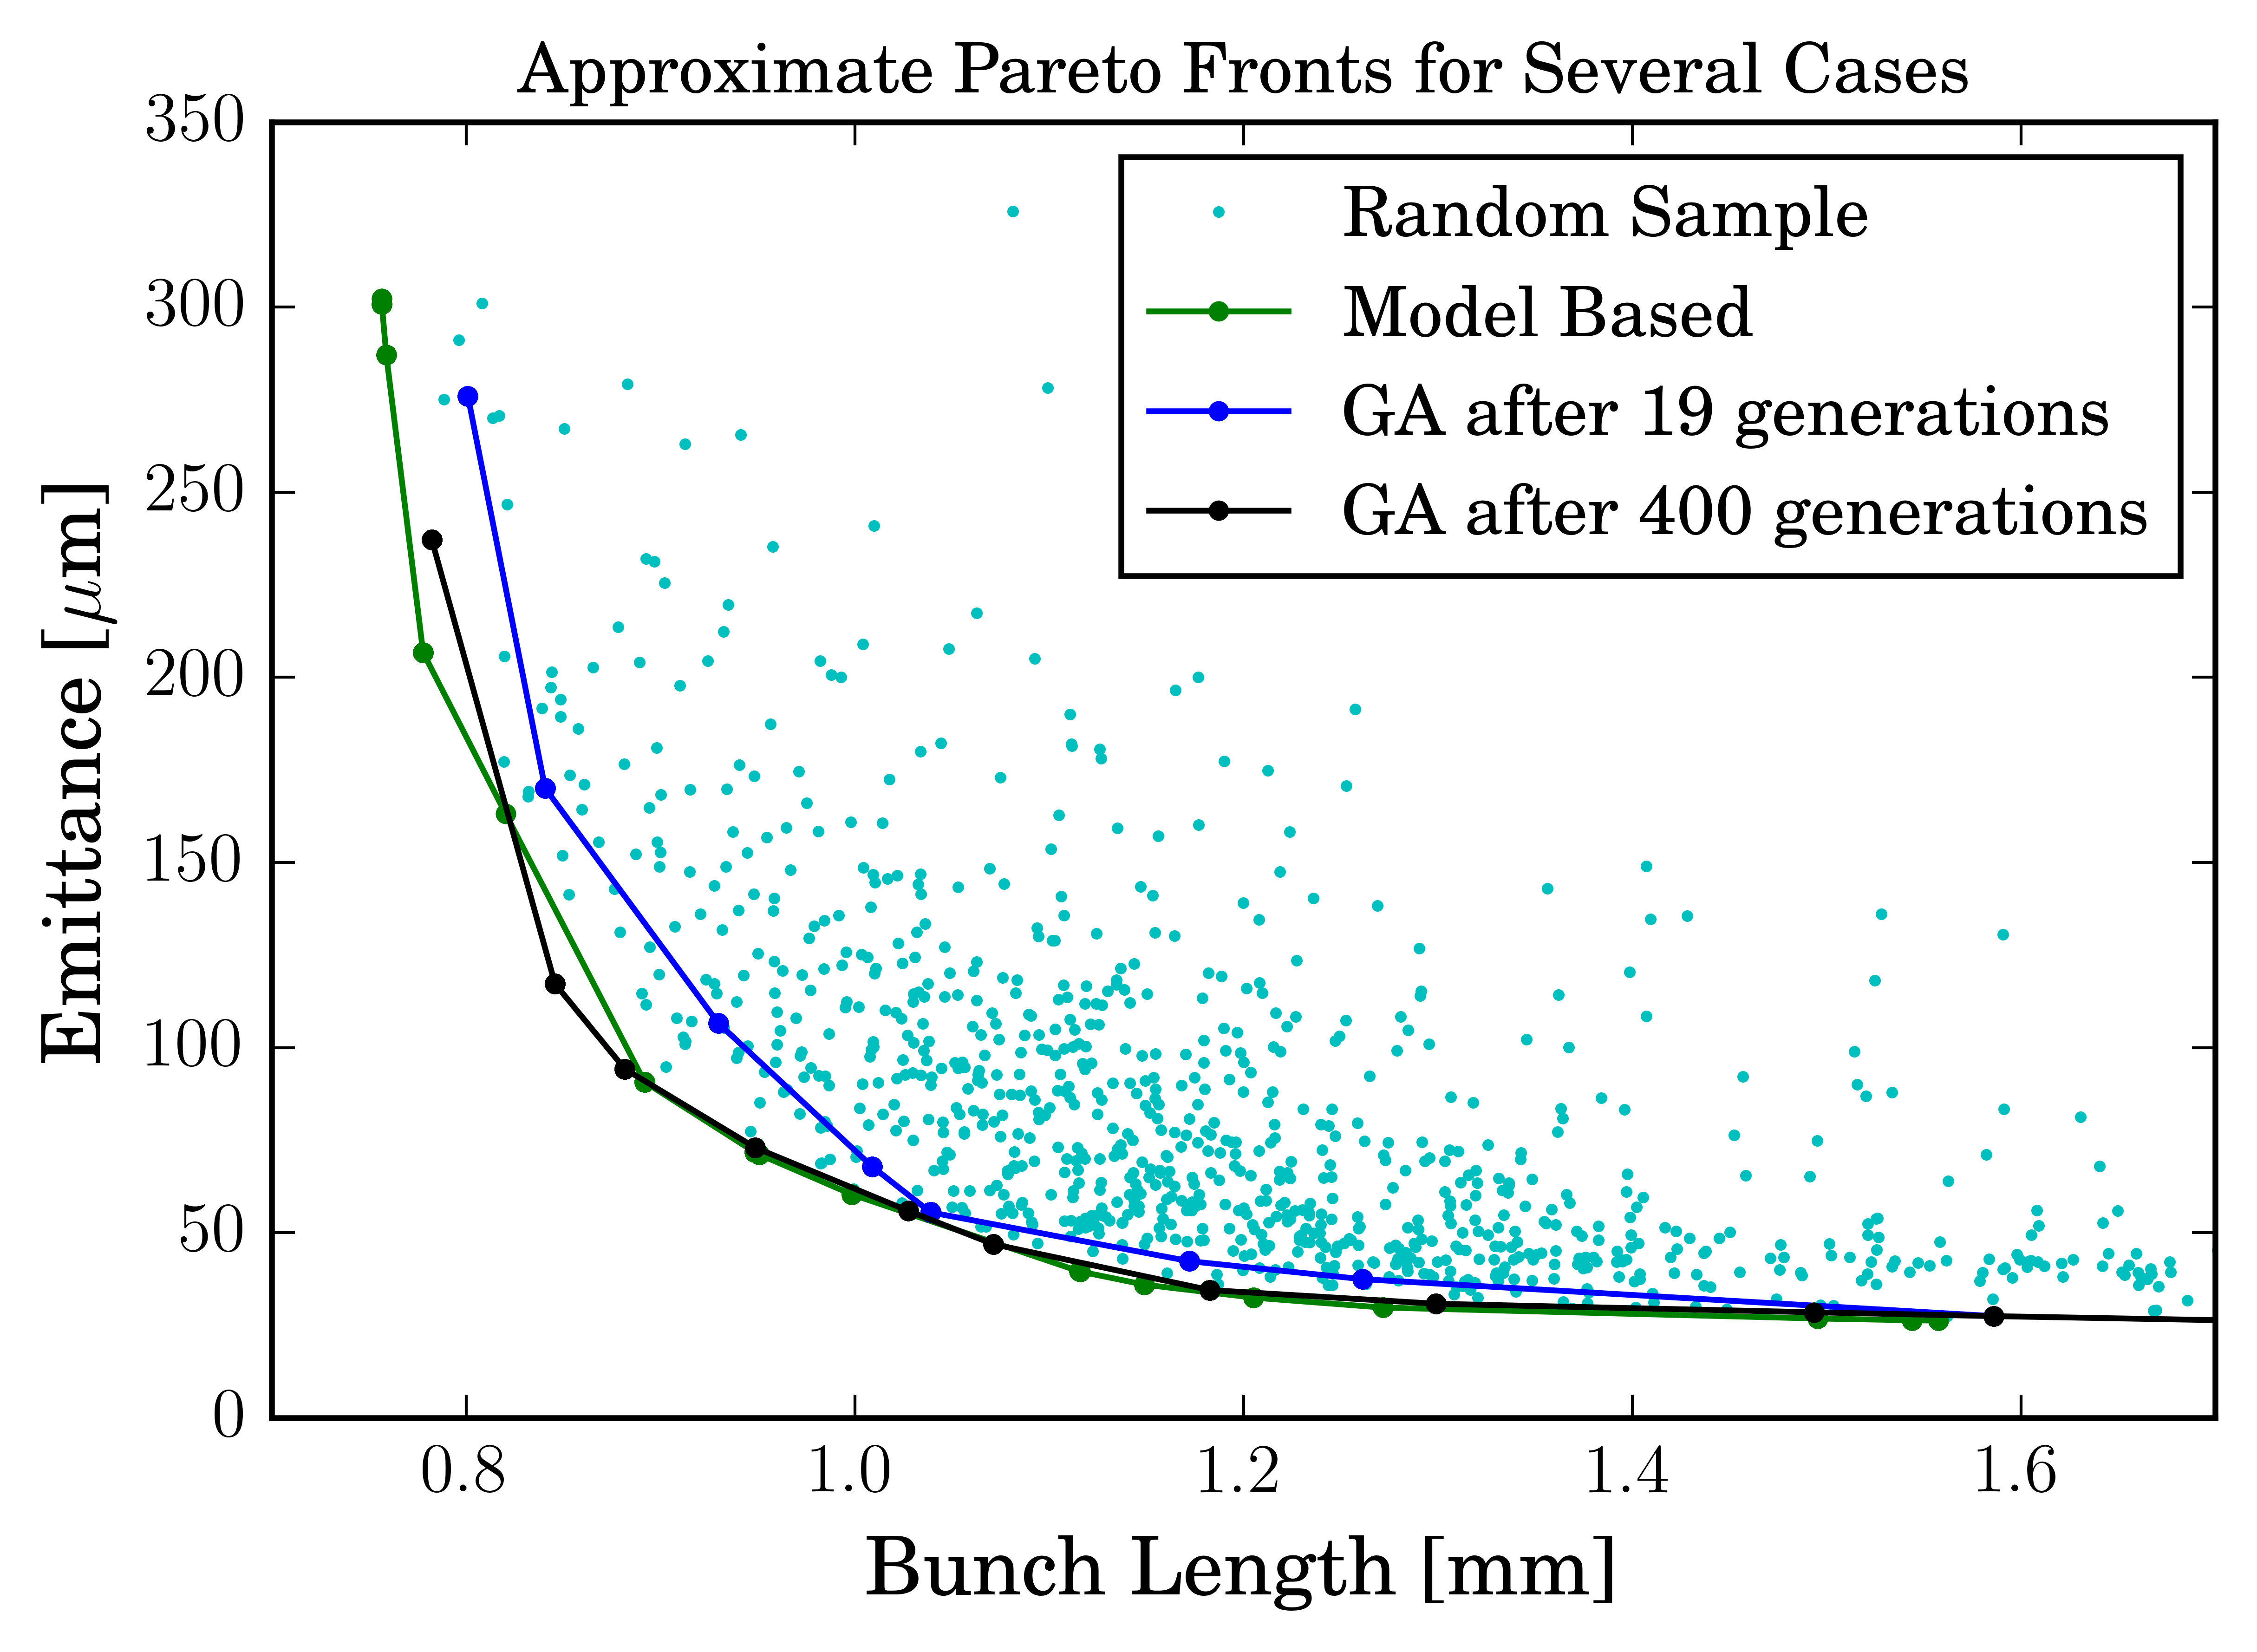
\includegraphics[width=0.65\linewidth]{../../tex/images/model_vs_ga}
\begin{itemize}
	\item 2,393 simulations for BOBYQA.
	\item 2,432 for 19 generation GA.
	\item 25,600 for 200 generation GA.
\end{itemize}
\end{frame}
}%end of simulations section
%%%%%%%%%%%%%%%%%%%%%%%%%%%%%%%%%%%%%%%%%%%%%%%%%%%%%%%%%%%%%%%%%%%%%%%%%%%%%%%
%%%%%%%%%%%%%%%%%%%%%%%%%%%%%%%%%%%%%%%%%%%%%%%%%%%%%%%%%%%%%%%%%%%%%%%%%%%%%%%%
%%%%%%%%%%%%%%%%%%%%%%%%%%%%%%%%%%%%%%%%%%%%%%%%%%%%%%%%%%%%%%%%%%%%%%%%%%%%%%%%%
%%%%%%%%%%%%%%%%%%%%%%%%%%%%%%%%%%%%%%%%%%%%%%%%%%%%%%%%%%%%%%%%%%%%%%%%%%%%%%%%%
\section{TBA Beam Line Design}
\begin{frame}
\frametitle{TBA Beam Line Under Design}
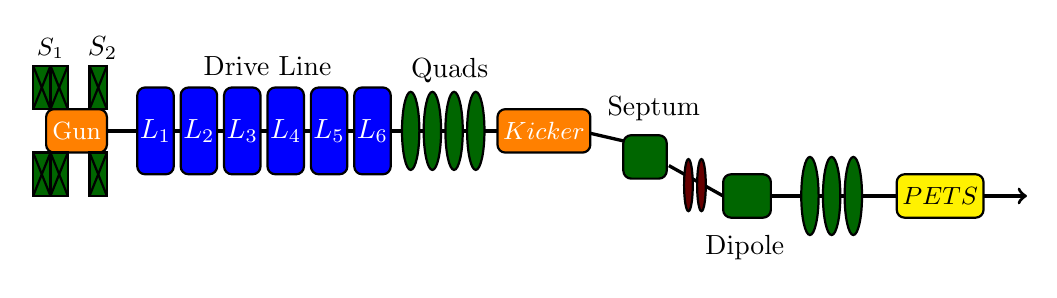
\begin{tikzpicture}[scale=\textwidth/22cm, text=black]
\def \gunleft {-1.0}
\def \gunright {0.3}
\def \loneright {1.0}
\def \ltworight {2.0}
\def \lthreeright {3.0}
\def \lfourright {4.0}
\def \lfiveright {5.0}
\def \lsixright {6.0}
\def \quadone {7.3}
\def \quadfour{16}

\draw[very thick, ->] (0.0,1) -- (10,1);

\draw[fill=orange, thick, rounded corners =0.1cm] (\gunleft-0.1,0.5)rectangle (\gunright,1.5) node[pos=.5, white] {\small{Gun}} ;
%Straight through

%S1
\node[] at (-1,2.9) {\small{$S_1$}};
\draw[thick, fill=black!60!green] (-1.4,-0.5)rectangle  (-1.0,0.5) node[pos=.5, white] {} ;
\draw[black,  thick] (-1.4,-0.5) -- (-1.0,0.5);
\draw[black,  thick] (-1.4,0.5) -- (-1.0,-0.5);
\draw[ thick, fill=black!60!green] (-1.4,1.5)rectangle  (-1.0,2.5) node[pos=.5, white] {} ;
\draw[black,  thick] (-1.4,1.5) -- (-1.0,2.5);
\draw[black,  thick] (-1.4,2.5) -- (-1.0,1.5);

\draw[ thick, fill=black!60!green] (-1.0,-0.5)rectangle  (-0.6,0.5) node[pos=.5, white] {} ;
\draw[black,  thick] (-1.0,-0.5) -- (-0.6,0.5);
\draw[black,  thick] (-1.0,0.5) -- (-0.6,-0.5);
\draw[ thick, fill=black!60!green] (-1.0,1.5)rectangle  (-0.6,2.5) node[pos=.5, white] {} ;
\draw[black,  thick] (-1.0,1.5) -- (-0.6,2.5);
\draw[black,  thick] (-1.0,2.5) -- (-0.6,1.5);

%S2
\node[] at (0.2,2.9) {$S_2$};
\draw[ thick, fill=black!60!green] (-0.1,-0.5) rectangle  (0.3,0.5) node[pos=.5, white] {};
\draw[black,  thick] (-0.1,-0.5) -- (0.3,0.5);
\draw[black,  thick] (-0.1,0.5) -- (0.3,-0.5);
\draw[ thick, fill=black!60!green] (-0.1,1.5) rectangle  (0.3,2.5) node[pos=.5, white] {};
\draw[black,  thick] (-0.1,1.5) -- (0.3,2.5);
\draw[black,  thick] (-0.1,2.5) -- (0.3,1.5);
%Linac drawings 
%\node[] at (4,2.5) {Accelerating Cavities};
\draw[fill=blue,  thick, rounded corners =0.1cm] (\loneright,0)rectangle  ({\loneright+0.84},2) node[pos=.5, white] {$L_1$} ;
\draw[fill=blue,  thick, rounded corners =0.1cm] (\ltworight,0)rectangle  ({\ltworight+0.84},2) node[pos=.5, white] {$L_2$};
\draw[fill=blue,  thick, rounded corners =0.1cm] (\lthreeright,0)rectangle ({\lthreeright+0.84},2) node[pos=.5, white] {$L_3$};
\draw[fill=blue,  thick, rounded corners =0.1cm] (\lfourright,0)rectangle ({\lfourright+0.84},2) node[pos=.5, white] {$L_4$};
\draw[fill=blue,  thick, rounded corners =0.1cm] (\lfiveright,0)rectangle ({\lfiveright+0.84},2) node[pos=.5, white] {$L_5$};
\draw[fill=blue,  thick, rounded corners =0.1cm] (\lsixright,0)rectangle ({\lsixright+0.84},2) node[pos=.5, white] {$L_6$};



%Quad drawings
\node[] at (8.2,2.4) {Quads};
\draw[fill=black!60!green,  thick] (\quadone, 1.0) ellipse (0.2cm and 0.9cm);
\draw[fill=black!60!green,  thick] (\quadone+0.5, 1.0) ellipse (0.2cm and 0.9cm);
\draw[fill=black!60!green,  thick] (\quadone+1.0, 1.0) ellipse (0.2cm and 0.9cm);
\draw[fill=black!60!green,  thick] (\quadone+1.5, 1.0) ellipse (0.2cm and 0.9cm);

%Line between kicker and septum
\node[] at (4,2.5) {Drive Line};
\draw[very thick] (\lsixright+5.2,1.0) -- (12.5,0.7);

%Kicker 
\draw[fill=orange,  thick, rounded corners =0.1cm] (\lsixright+3.3,0.5)rectangle ({\lsixright+0.84+4.6},1.5) node[pos=.5, white] {\small{$Kicker$}};

%Septum
\node[] at (12.9,1.5) {Septum};
\draw[fill=black!60!green,  thick, rounded corners =0.1cm] (12.2,0.9)rectangle ({13.2},-0.1) node[pos=.5, white] {};
%\draw[latex-latex] (\gunleft,-5.0) -- (14,-5.0) ;
%\foreach \x in  {0.3, 1.0, 3.5, 5.0, 7.0, 8.5, 10, 12.5} %tick marks
%\draw[shift={(\x,-5.0)},color=black] (0pt,3pt) -- (0pt,-3pt);
%\foreach \x in {0.3, 1.0, 3.5, 5.0, 7.0, 8.5, 10, 12.5}
%\draw[shift={(\x,-5.2)},color=black] (0pt,0pt) node[below] {$\x$};

%Line between kicker and septum
\draw[very thick] (13.25,0.2) -- (14.5,-0.5);

%Second set of quads
\draw[fill=black!60!red,  thick] (\quadfour-2.3, -0.250) ellipse (0.1cm and 0.6cm);
\draw[fill=black!60!red,  thick] (\quadfour-2, -0.250) ellipse (0.1cm and 0.6cm);

%Dipole
\node[] at (15,-1.7) {Dipole};
\draw[fill=black!60!green, thick, rounded corners =0.1cm] (14.5,0.0)rectangle ({15.6},-1.0) node[pos=.5, white] {};

%Line between dipole and quads
\draw[very thick, ->] (15.6,-0.5) -- (21.5,-0.5);
%Second set of quads
\draw[fill=black!60!green,  thick] (\quadfour+0.5, -0.50) ellipse (0.2cm and 0.9cm);
\draw[fill=black!60!green,  thick] (\quadfour+1.0, -0.50) ellipse (0.2cm and 0.9cm);
\draw[fill=black!60!green,  thick] (\quadfour+1.5, -0.50) ellipse (0.2cm and 0.9cm);

%Kicker 
\draw[fill=yellow,  thick, rounded corners =0.1cm] (\quadfour+2.5,0)rectangle ({\quadfour+4.5},-1) node[pos=.5, black] {\small{$PETS$}};






\end{tikzpicture}

\vspace{-1.5em}

Requirements and Mechanical Constraints:
\begin{itemize}
	\item 100\% transmission, i.e. reasonable beam size at structure
	\item Reasonable bunch length at structure (maximize power)
	\item 1m between kicker and septum
	\begin{itemize}
		\item for separation $\ge$ 50mm in septum. 
	\end{itemize}
	\item 1.8m between septum and dipole
	\begin{itemize}
		\item for separation $\ge$ 0.5m of beam lines.
	\end{itemize}
	\item 15cm between quads for easy installation. 
	\item 0.3m between quads and PETS for yag screen.  
\end{itemize}
\end{frame}

\begin{frame}
	\frametitle{GA applied to TBA Beam Line}
	\begin{center}
		\setcounter{mpfootnote}{\value{footnote}}%
		\renewcommand{\thempfootnote}{\arabic{mpfootnote}}%	
		\begin{tabular}{ l *{3}{c}}
			%\toprule
			\textbf{Variable} & \textbf{Range} & \textbf{Unit} \\
			\midrule
			Buck Focusing Solenoid Strength & $ 300 \le S_3 \le 500$  & amps \\
			Matching Solenoid Strength & $ 180 \le S_3 \le 280$  & amps \\
			Quadrupole Strength  & $-8.0 \le K_i$\footnote[1]{$K_i=[K_{1},\ldots,K_{4}]$}  $\le 8.0$ & T/m \\
			%\bottomrule    
		\end{tabular}
	\end{center}
\begin{minipage}{0.4\textwidth}
	\textbf{Simulation Inputs:}
	\begin{itemize}
		\item 6 design variables
		\item Laser radius is 9 cm
		\item Laser FWHM 10 ps
		\item All cavities at $-20^\circ$
	\end{itemize}
\end{minipage}
\begin{minipage}{0.55\textwidth}
	\textbf{Objectives:}
	\begin{itemize}
		\item Transverse beam size, $\sigma_{x,y}$
		\item Transverse momentum, $\sigma_{px,py}$
		\item Bunch length, $\sigma_z$
		\item Energy spread, dE
	\end{itemize}
\end{minipage}
\end{frame}

\begin{frame}
	\frametitle{OPAL GA Code: Variables}
	\centering
	\Wider[8em]{\tiny\lstVars}
\end{frame}
\begin{frame}
\frametitle{OPAL GA Code: Objectives}
\centering
\tiny\lstObjs
\end{frame}
\begin{frame}
\frametitle{OPAL GA Code: Simulations}
\begin{center}
	\Wider[8em]{\tiny\lstinfo}
\end{center}

\end{frame}

\subsection{Results}
\begin{frame}
	\frametitle{TBA Pareto Fronts}
	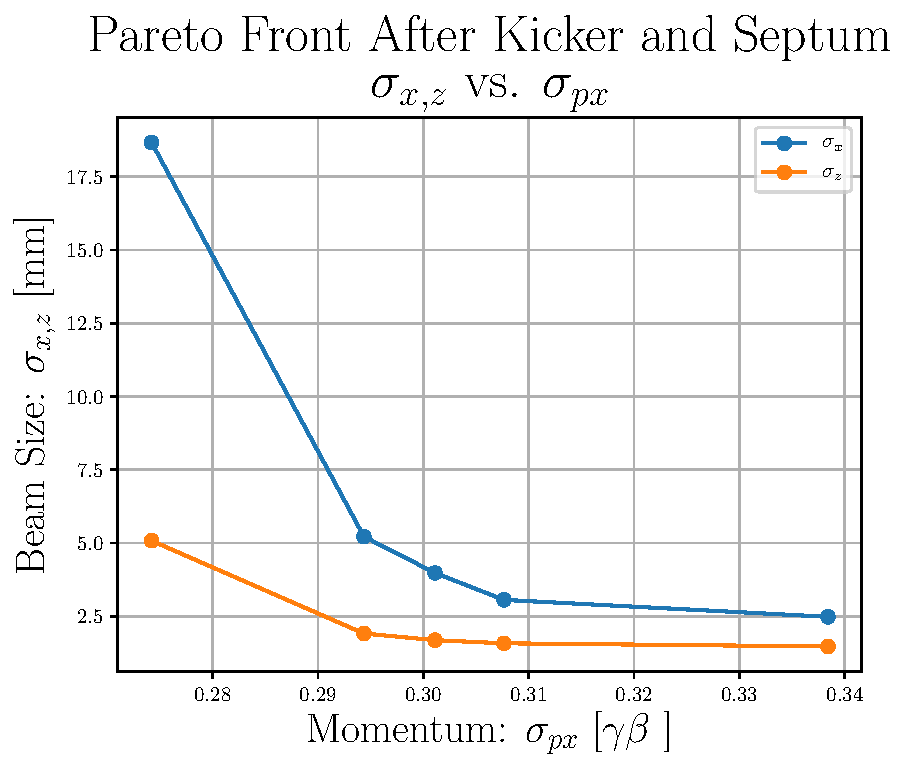
\includegraphics[width=0.5\textwidth]{../../tex/images/xz_vs_px_pareto_front_Q5}%
	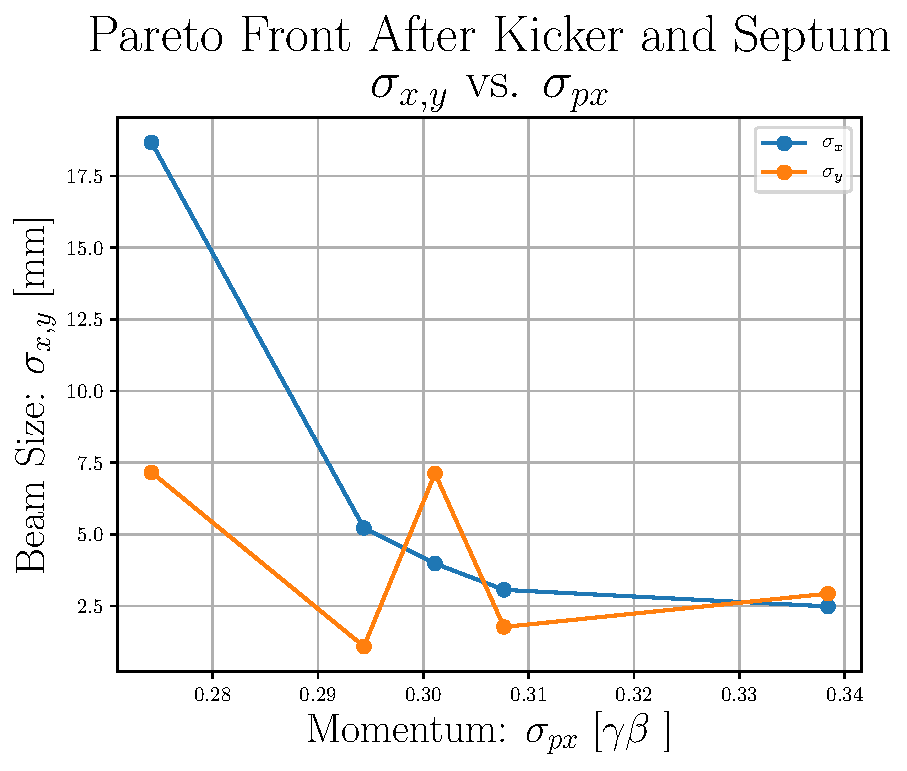
\includegraphics[width=0.5\textwidth]{../../tex/images/xy_vs_px_pareto_front_Q5}%
	\begin{itemize}
		\item Looking at entrance of 5th quad
		\item Location between septum and dipole
		\item Optimizing here will reduce beam size growth in dipole
	\end{itemize}
\end{frame}

\begin{frame}
	\frametitle{Beam Size Results in Optimized Solutions}
	\vspace{-1em}
	\begin{center}
		\Wider[4em]{
			\centering
		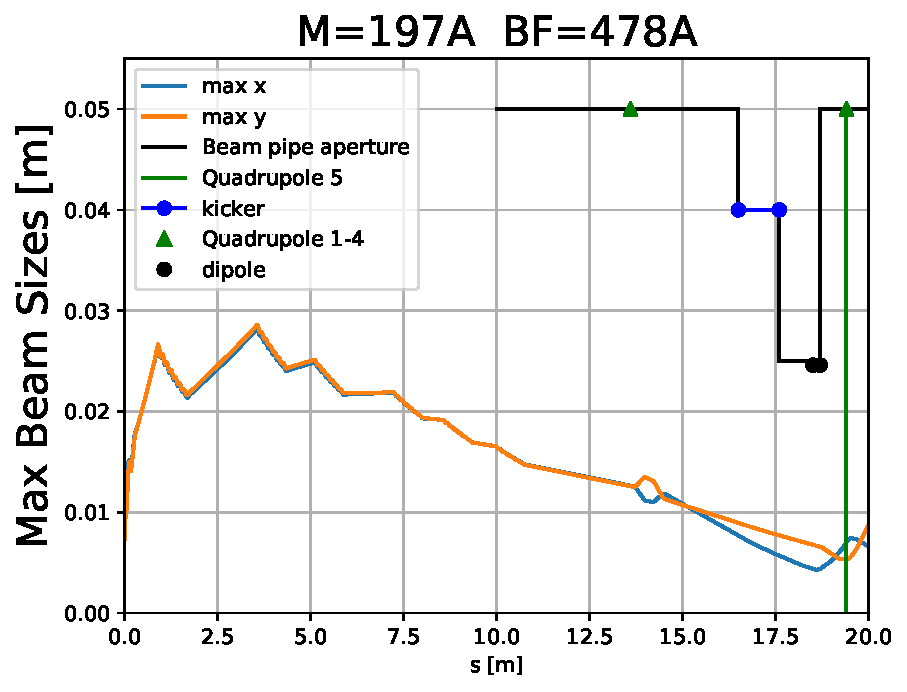
\includegraphics[width=0.35\textwidth]{{../../tex/images/xy-max-min-optLinac-40nC_IM=197_IBF=478_KQ1=-0.8_KQ2=0.9_KQ3=0.8_KQ4=-1.0.stat}.pdf}%
		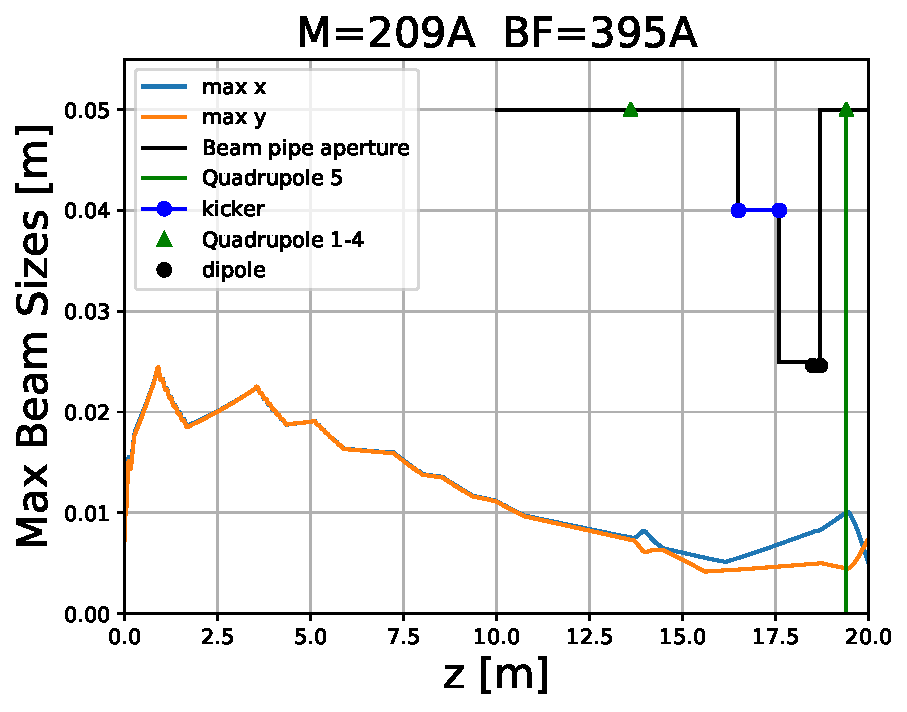
\includegraphics[width=0.35\textwidth]{{../../tex/images/xy-max-min-optLinac-40nC_IM=209_IBF=395_KQ1=1.1_KQ2=-1.88_KQ3=0.39_KQ4=0.61.stat}.pdf} \\
		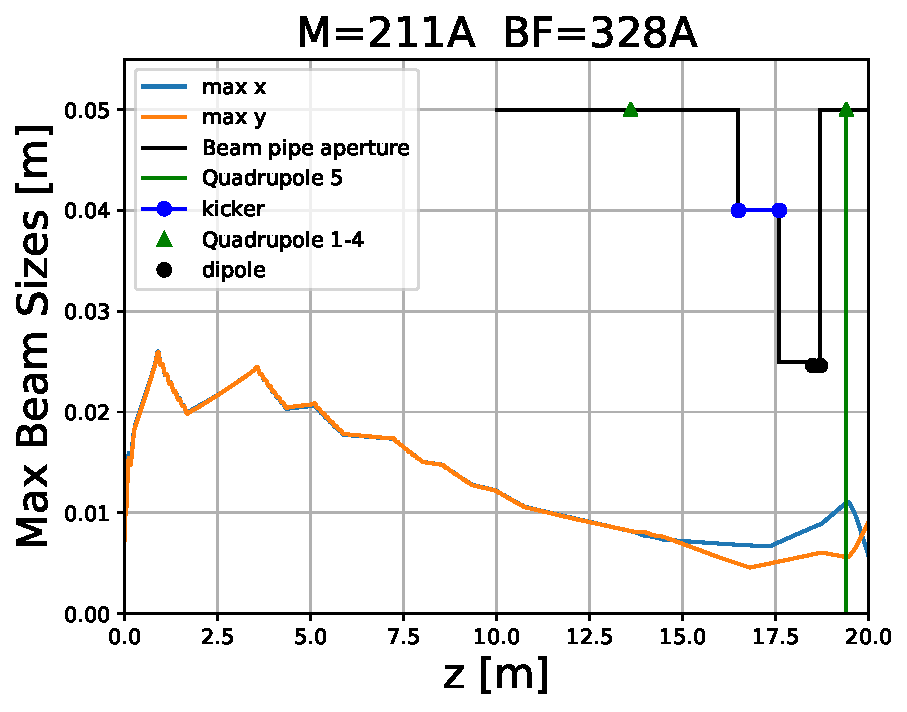
\includegraphics[width=0.35\textwidth]{{../../tex/images/xy-max-min-optLinac-40nC_IM=211_IBF=328_KQ1=-0.21_KQ2=0.37_KQ3=-0.26_KQ4=0.25.stat}.pdf}%
		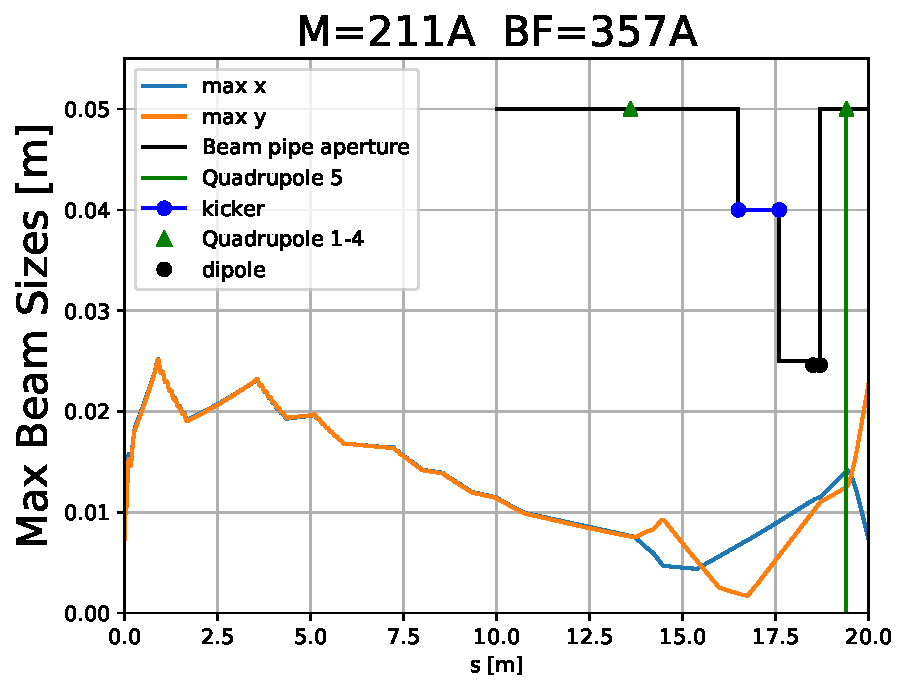
\includegraphics[width=0.35\textwidth]{{../../tex/images/xy-max-min-optLinac-40nC_IM=211_IBF=357_KQ1=-0.72_KQ2=0.2_KQ3=-0.73_KQ4=1.92.stat}.pdf}
	}
	\end{center}
\end{frame}

\begin{frame}
\vspace{-1em }
\frametitle{Best Solution}
\tiny
\begin{minipage}{0.6\textwidth}
	\begin{itemize}
			\item Symmetric beam not necessary, if transmission is good.
			\item PETS aperture = 17.6 mm
			\item Need to adjust matching and quads.
			\item Energy $\approx$ 65 MeV
	\end{itemize}
\end{minipage}
\begin{minipage}{0.35\textwidth}
	\begin{table}[hbt] 
		\centering
		\begin{tabular}{ l *{3}{c}}
			\toprule
			\textbf{Quad} &  \textbf{Value} & \textbf{Unit} \\
			\midrule
			Q1	  & -0.8 & amps \\
			Q2 	  & 0.9  & amps \\
			Q3	  & 0.8  & amps \\
			Q4    & -1.0 & amps \\
			\bottomrule	
		\end{tabular}	
	\end{table}	
\end{minipage}

\vspace{1em}

\begin{minipage}{0.49\textwidth}
\centering	
2D Field Maps only \\
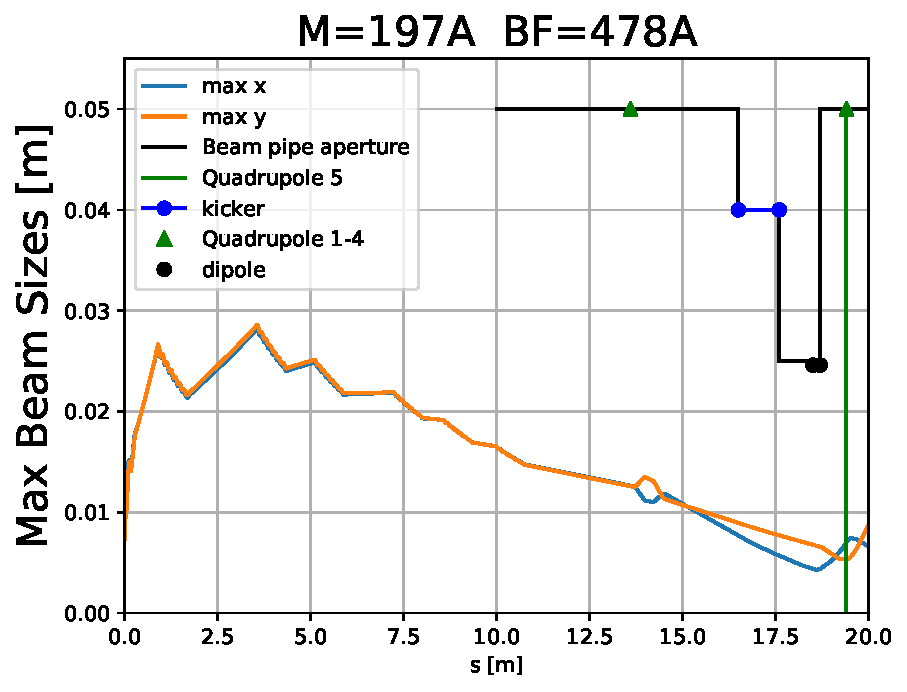
\includegraphics[width=\textwidth]{{../../tex/images/xy-max-min-optLinac-40nC_IM=197_IBF=478_KQ1=-0.8_KQ2=0.9_KQ3=0.8_KQ4=-1.0.stat}.pdf}	
\end{minipage}
\begin{minipage}{0.49\textwidth}
\centering
3D Maps and CSR included \\
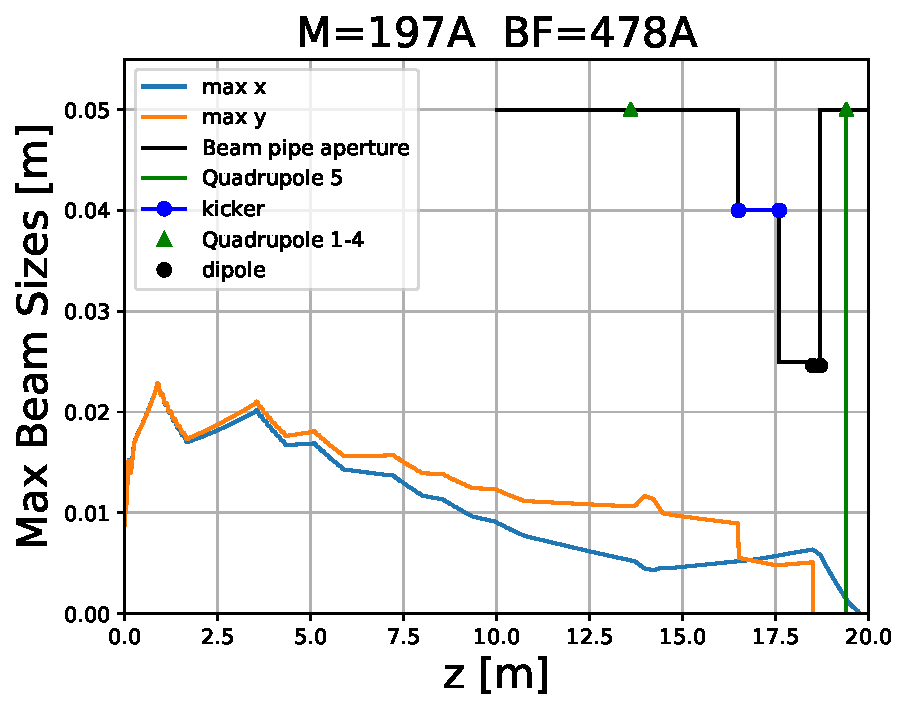
\includegraphics[width=\textwidth]{{../../tex/images/xy-max-min-optLinac-40nC_IM=197_IBF=478_KQ1=-0.8_KQ2=0.9_KQ3=0.8_KQ4=-1.0_KQ5=-2.0_KQ6=1.25_CSR.stat}.pdf}		
\end{minipage}
\end{frame}

\begin{frame}
	\frametitle{Adjusted 3D/CSR Solution}
		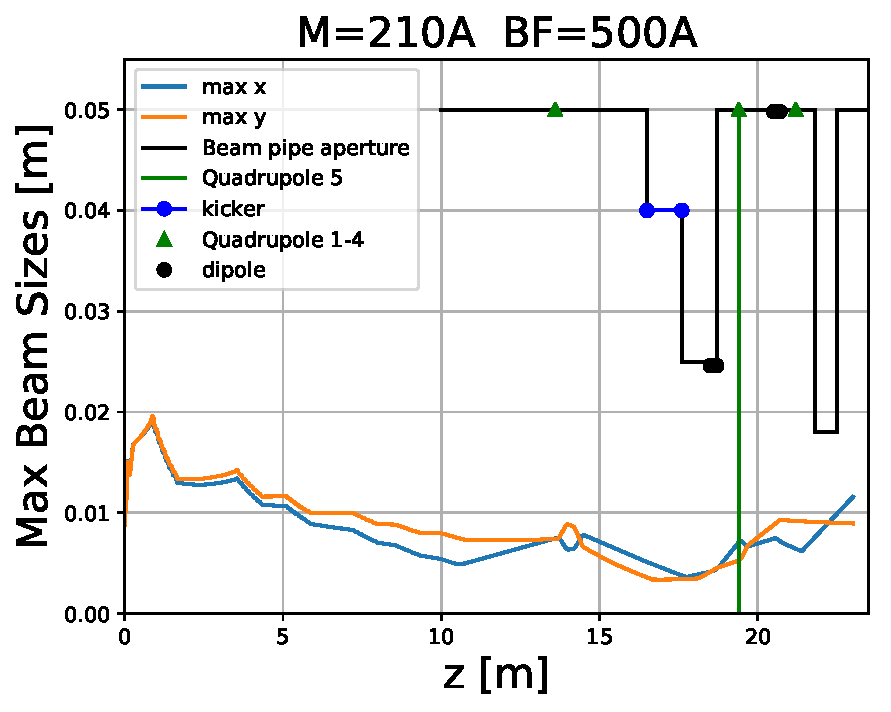
\includegraphics[width=0.5\textwidth]{{../../tex/images/xy-max-min-csr_optLinac-40nC_IM=210_IBF=500_KQ1=-1.5_KQ2=1.6_KQ3=1.5_KQ4=-1.7_KQ5=-2.0_KQ6=1.25.stat}.pdf}%
	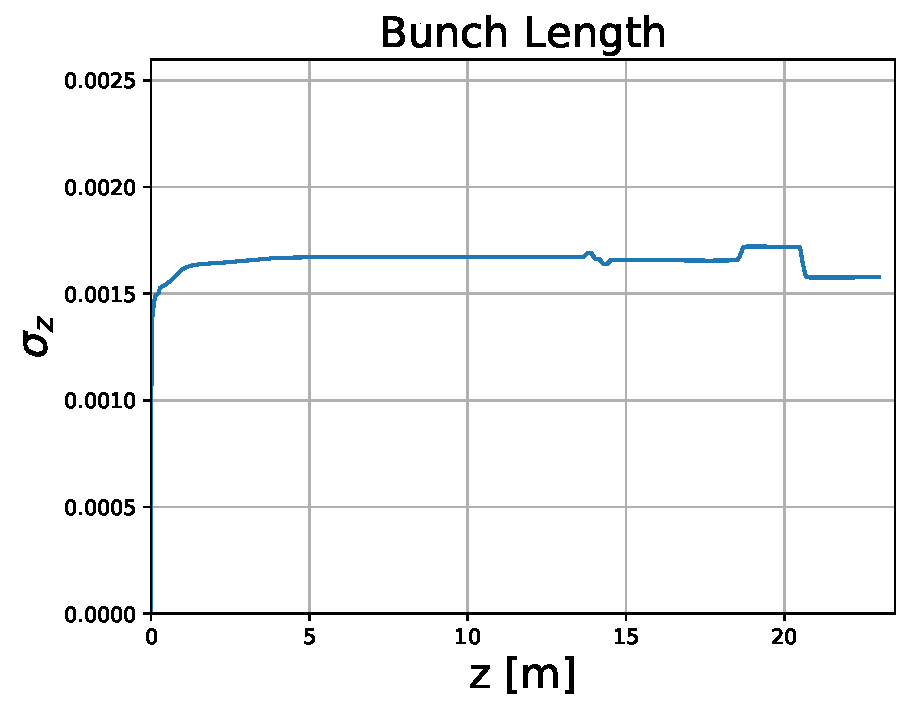
\includegraphics[width=0.5\textwidth]{{../../tex/images/zrms-csr_optLinac-40nC_IM=210_IBF=500_KQ1=-1.5_KQ2=1.6_KQ3=1.5_KQ4=-1.7_KQ5=-2.0_KQ6=1.25.stat}.pdf}
	
	\tiny
	\begin{minipage}{0.5\textwidth}
		\begin{table} 
		\centering
		\begin{tabular}{ l *{3}{c}}
			\toprule
			\textbf{Quad} &  \textbf{Value} & \textbf{Unit} \\
			\midrule
			Q1	  & -1.5 & amps \\
			Q2 	  & 1.6  & amps \\
			Q3	  & 1.5  & amps \\
			Q4    & -1.7 & amps \\
			\bottomrule	
		\end{tabular}	
	\end{table}	
\end{minipage}
	\begin{minipage}{0.4\textwidth}
	\begin{itemize}
		\item Strengthened all quads by 0.7 A
		\item Last triplet not used!!!
	\end{itemize}
\end{minipage}
\end{frame}

\begin{frame}
	\frametitle{Movies!}
\end{frame}
%%%%%%%%%%%%%%%%%%%%%%%%%%%%%%%%%%%%%%%%%%%%%%%%%%%%%%%%%%%%%%%%%%%%%%%%%%%%%%%
%%%%%%%%%%%%%%%%%%%%%%%%%%%%%%%%%%%%%%%%%%%%%%%%%%%%%%%%%%%%%%%%%%%%%%%%%%%%%%%%
%%%%%%%%%%%%%%%%%%%%%%%%%%%%%%%%%%%%%%%%%%%%%%%%%%%%%%%%%%%%%%%%%%%%%%%%%%%%%%%%%
%%%%%%%%%%%%%%%%%%%%%%%%%%%%%%%%%%%%%%%%%%%%%%%%%%%%%%%%%%%%%%%%%%%%%%%%%%%%%%%%%
%%%%%%%%%%%%%%%%%%%%%%%%%%%%%%%%%%%%%%%%%%%%%%%%%%%%%%%%%%%%%%%%%%%%%%%%%%%%%%%%%
{
	\renewcommand{\secimage}{../../tex/images/YAG_screen}
\section{Experimental Measurements}
\begin{frame}
\frametitle{Beam Sizes}
Rewrote AWA Matlab script in python.
\begin{itemize}
	\item Fiducial calculation
	\item Background subtraction 
	\item Fitting functions; Gaussian and piece wise
\end{itemize}	

\vspace{1em}
\centering
\includegraphics[width=0.415\textheight]{/home/nicole/Documents/presentations/space_charge_2017/laser}%
\includegraphics[width=0.415\textheight]{/home/nicole/Documents/presentations/space_charge_2017/YAG2}%
\includegraphics[width=0.415\textheight]{/home/nicole/Documents/presentations/space_charge_2017/YAG3}
\end{frame}

\begin{frame}[t]
\frametitle{Matching Solenoid Scans}
\begin{columns}[T]
\begin{column}{0.76\textwidth}
\begin{minipage}{0.5\textheight}
	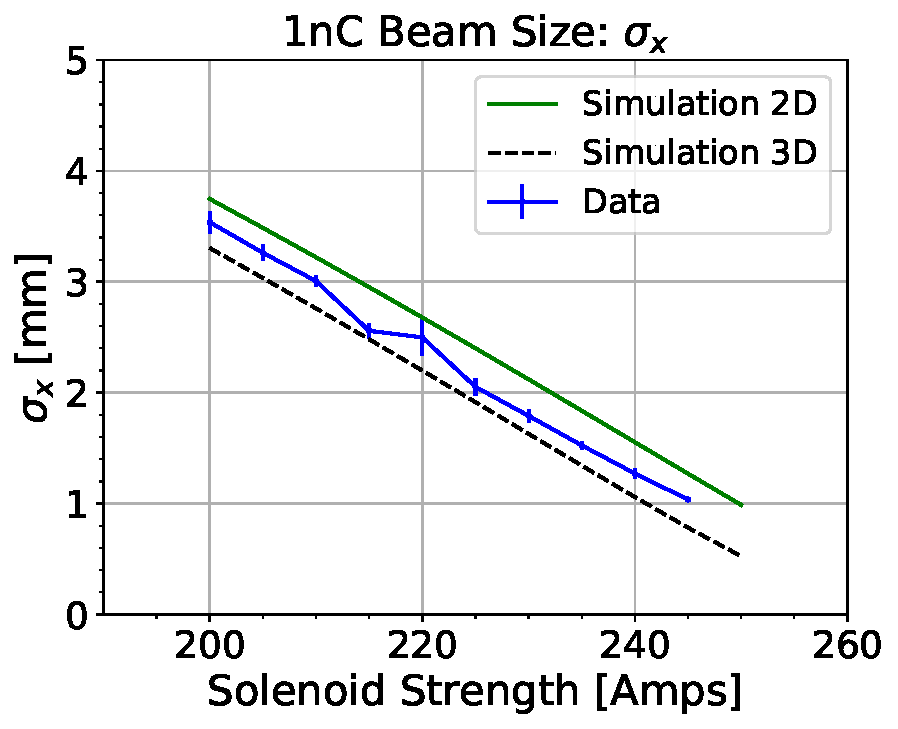
\includegraphics[width=1.0\linewidth]{../../tex/images/xbeamsizes_low_charge_sol_scan_11-02-2017}	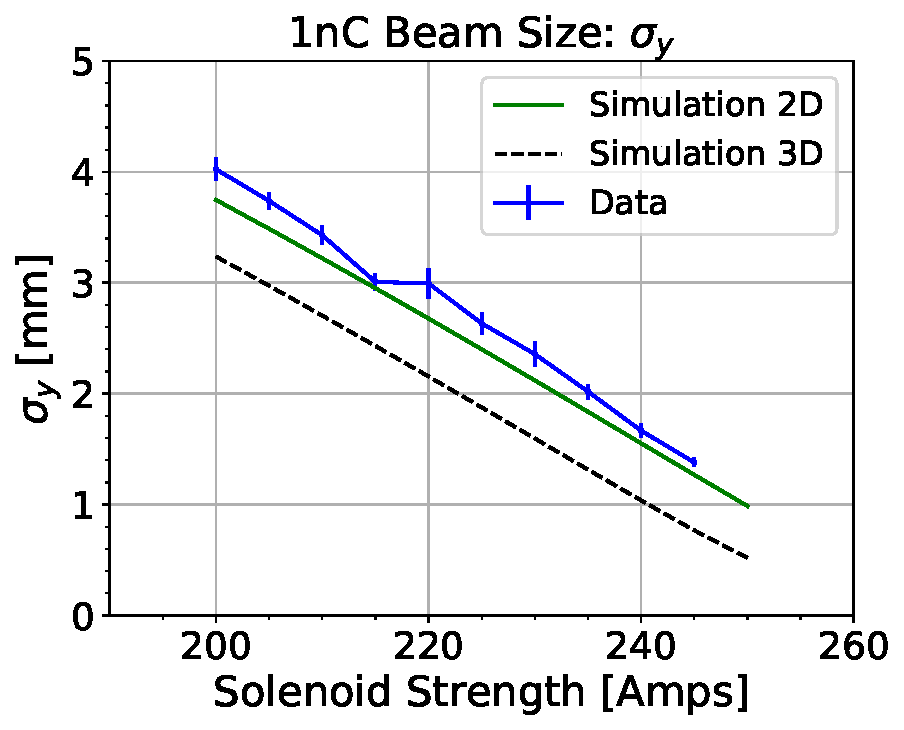
\includegraphics[width=1.0\linewidth]{../../tex/images/ybeamsizes_low_charge_sol_scan_11-02-2017}
\end{minipage}
\begin{minipage}{0.5\textheight}
	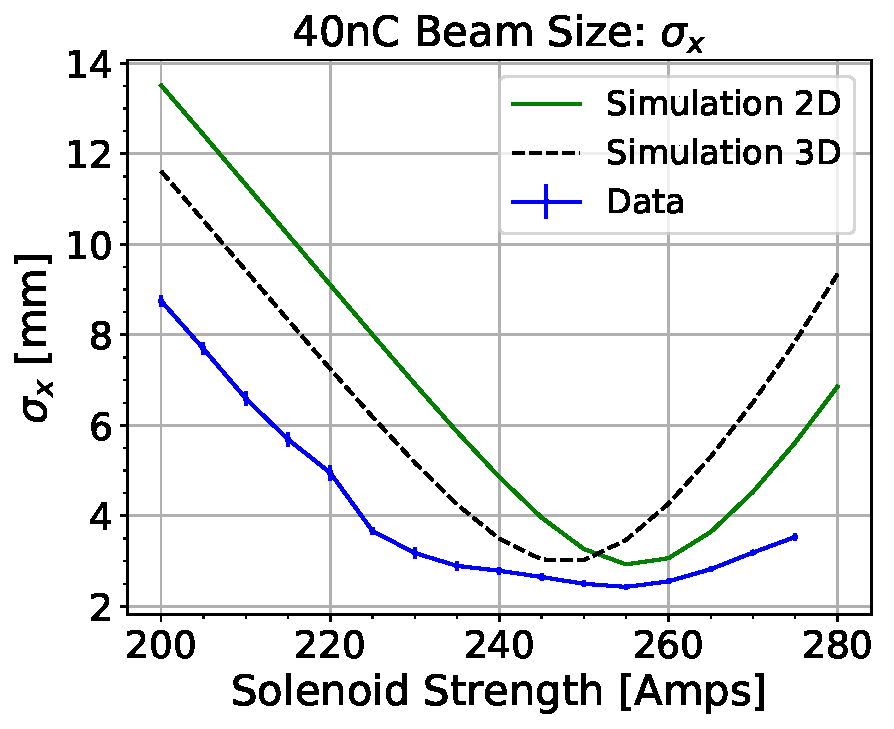
\includegraphics[width=1.0\linewidth]{../../tex/images/xbeamsizes_high_charge_sol_scan_10-17-2017}
	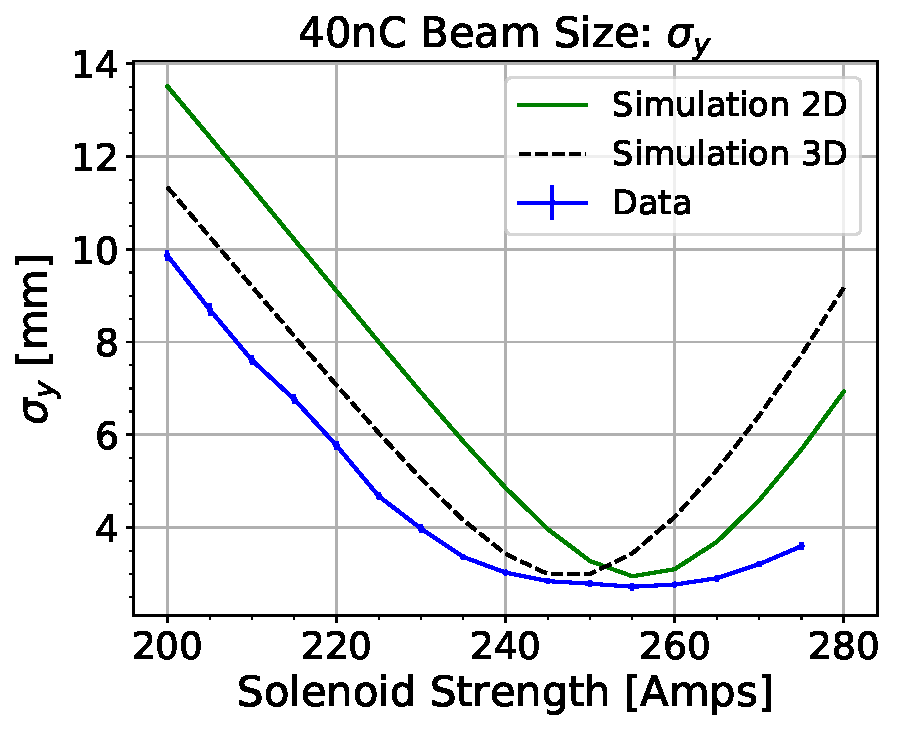
\includegraphics[width=1.0\linewidth]{../../tex/images/ybeamsizes_high_charge_sol_scan_10-17-2017}
\end{minipage}
\end{column}
\begin{column}{0.4\textwidth}
%\vspace{-9em}
\begin{itemize}
	\item only charge fluctuations are considered in error bars 
	\item Radius probably needs to be adjusted in simulations of high charge
\end{itemize}
\end{column}
\end{columns}
\end{frame}

\begin{frame}
\frametitle{Bunch Length Measurements}
Used Michelson interferometer and CTR light.
\centering
\Wider[4em]{
	\begin{minipage}{0.5\textwidth}
		\centering
		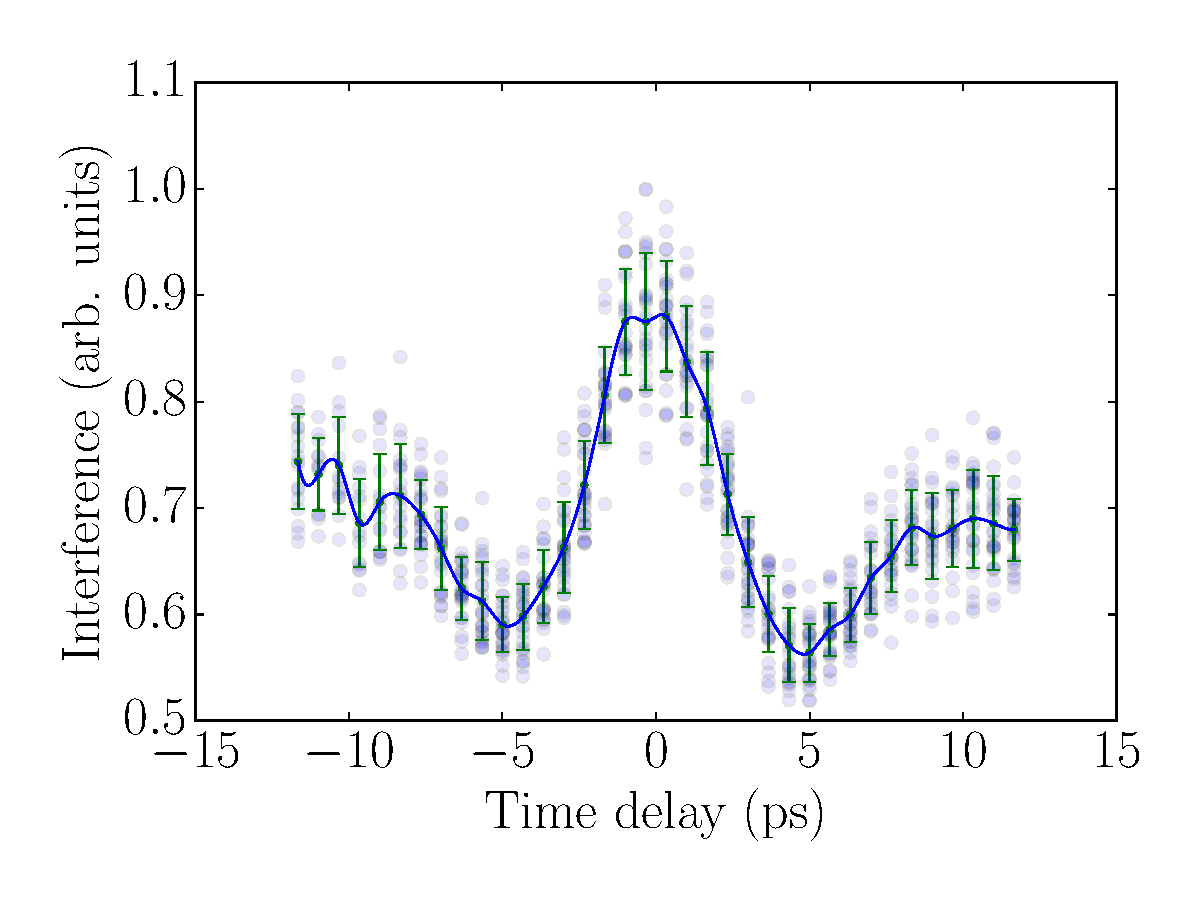
\includegraphics[width=0.7\textwidth]{../../tex/images/THPMF048f1}\\
		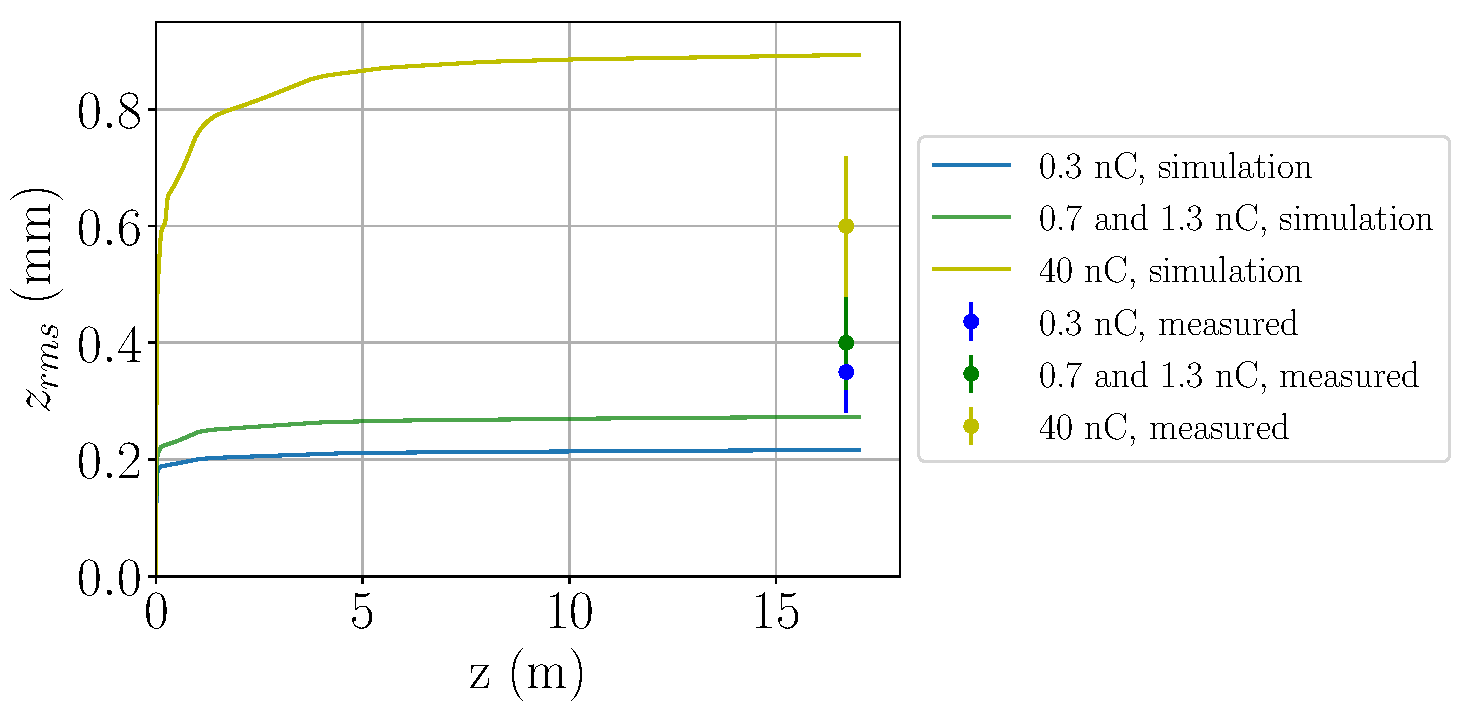
\includegraphics[width=\textwidth]{../../tex/images/THPMF048f5}
	\end{minipage}\hspace{1em}
	\begin{minipage}{0.4\textwidth}
		\centering
		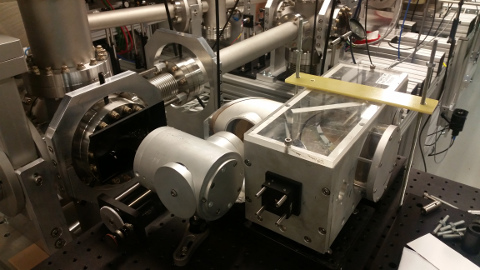
\includegraphics[width=\textwidth]{../../tex/images/THPMF048f3}
	\end{minipage}
}
\end{frame}
\subsection{Kicker}
\begin{frame}
	\frametitle{Kicker Fabrication}
	\centering
	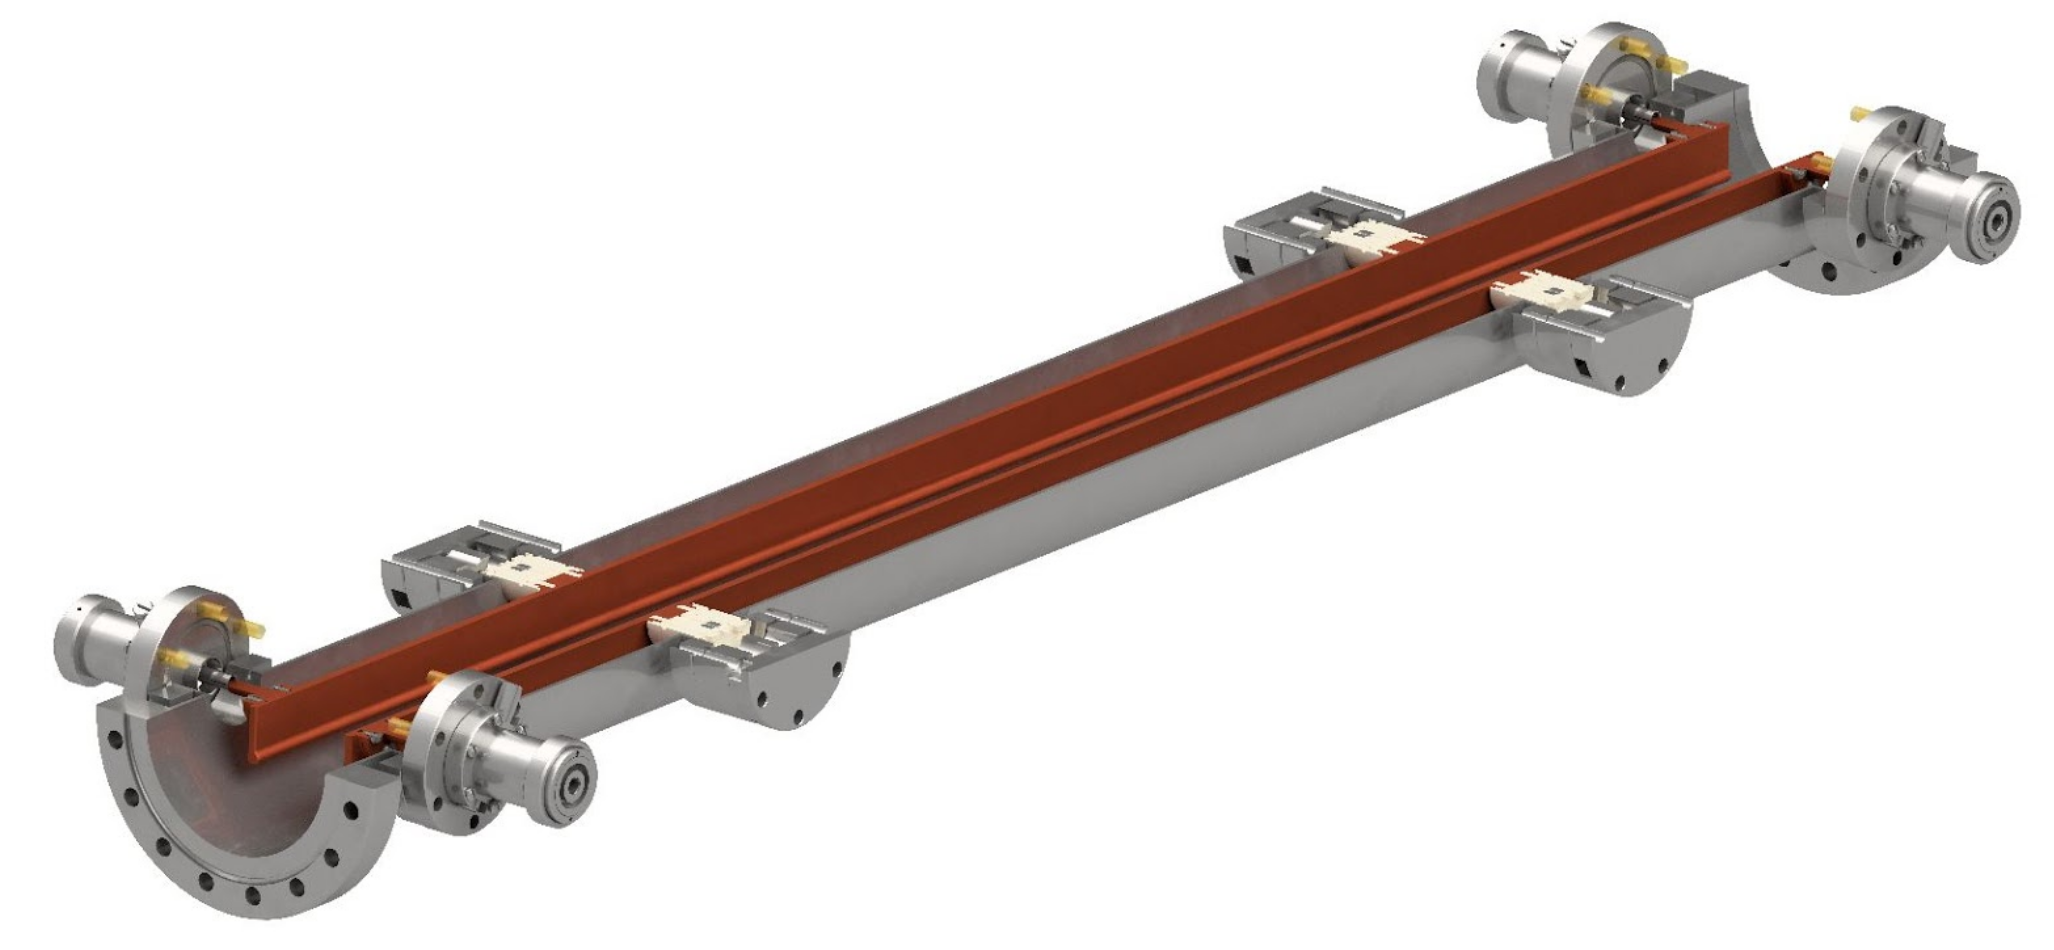
\includegraphics[width=0.7\textwidth]{../../tex/images/kicker}\\
	\tiny{*CAD drawing courtesy Scott Doran}
	\vspace{1em}
	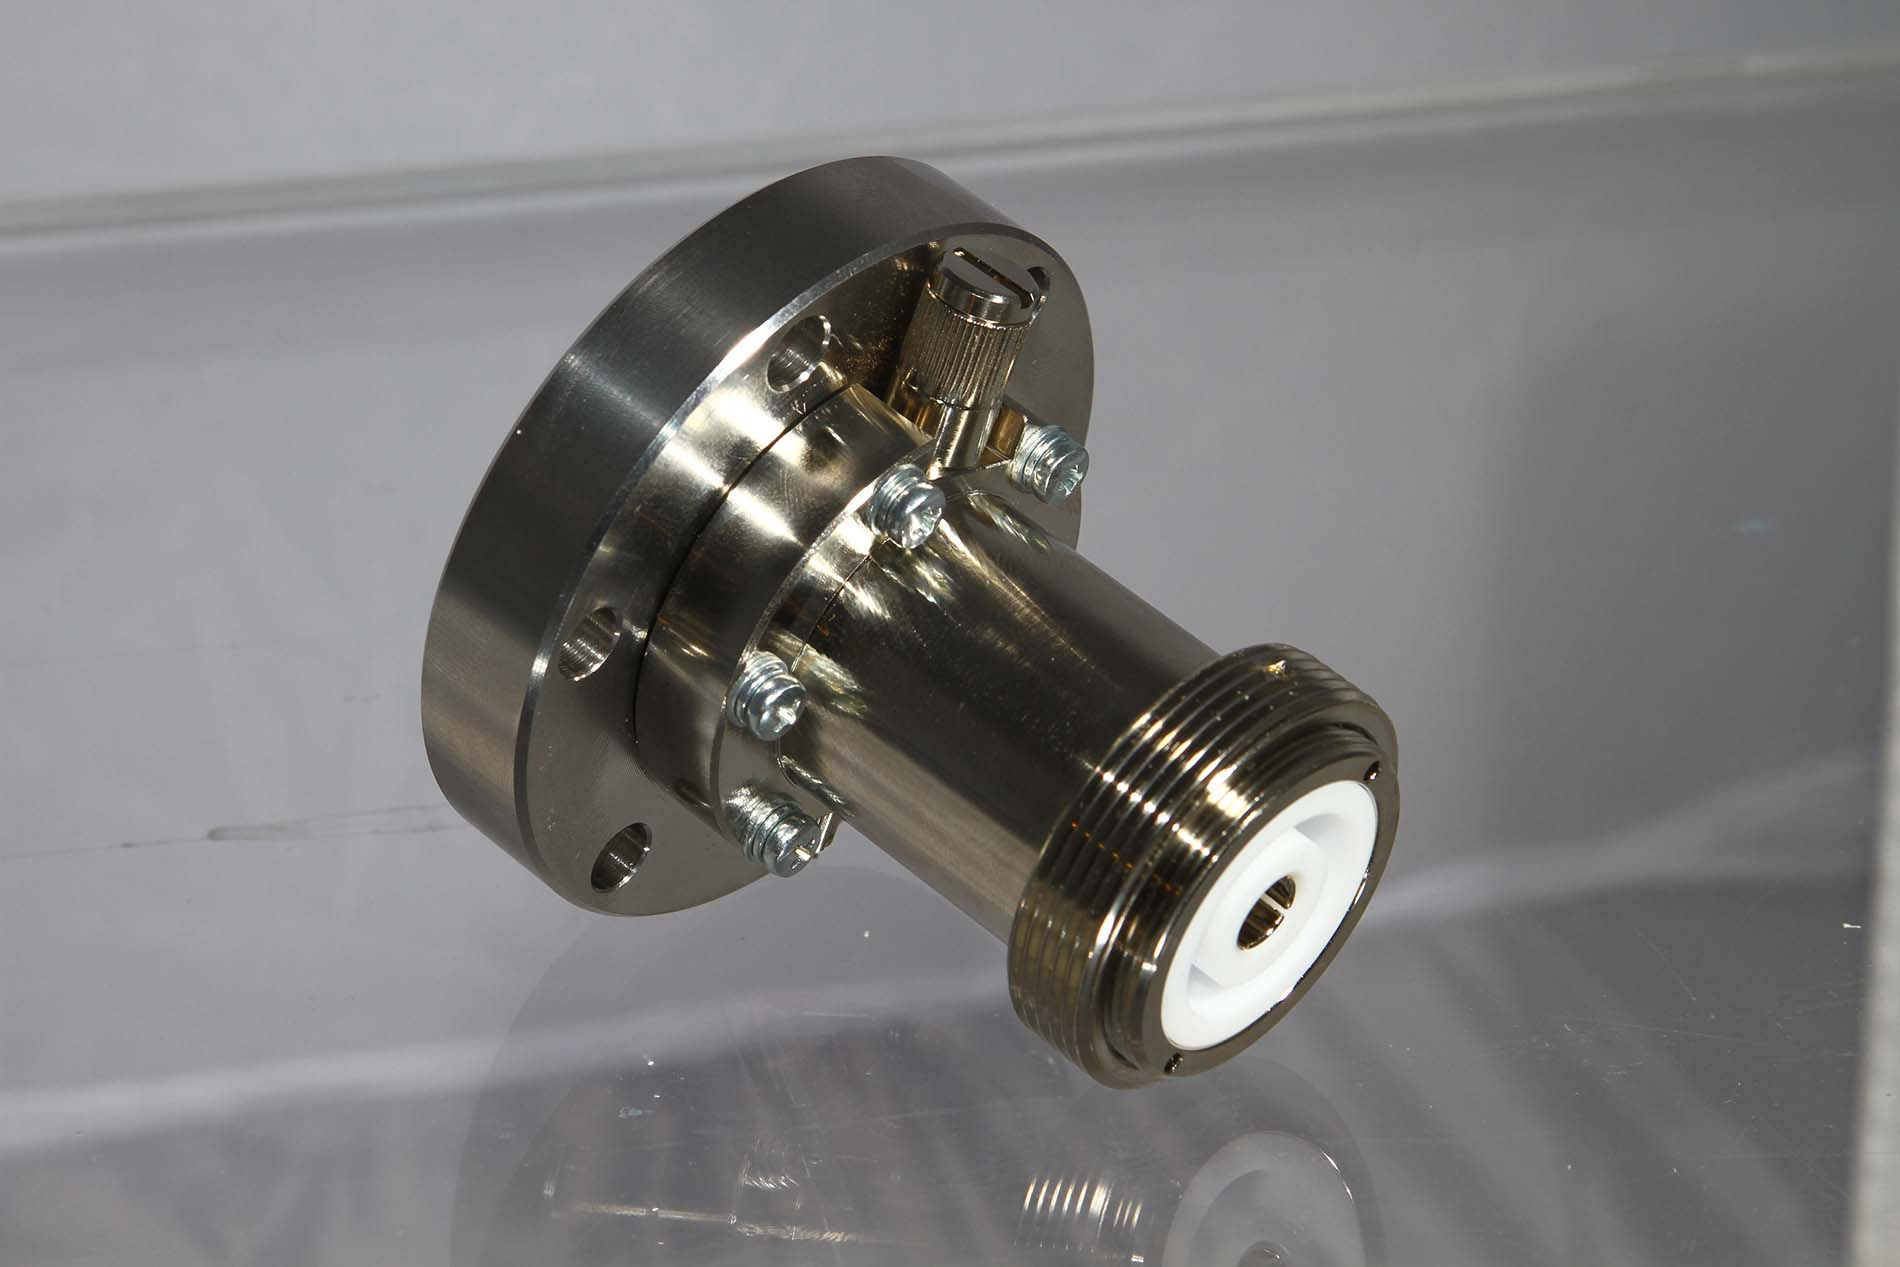
\includegraphics[width=0.33\textwidth]{../../tex/images/FID_feedthrough1}%
	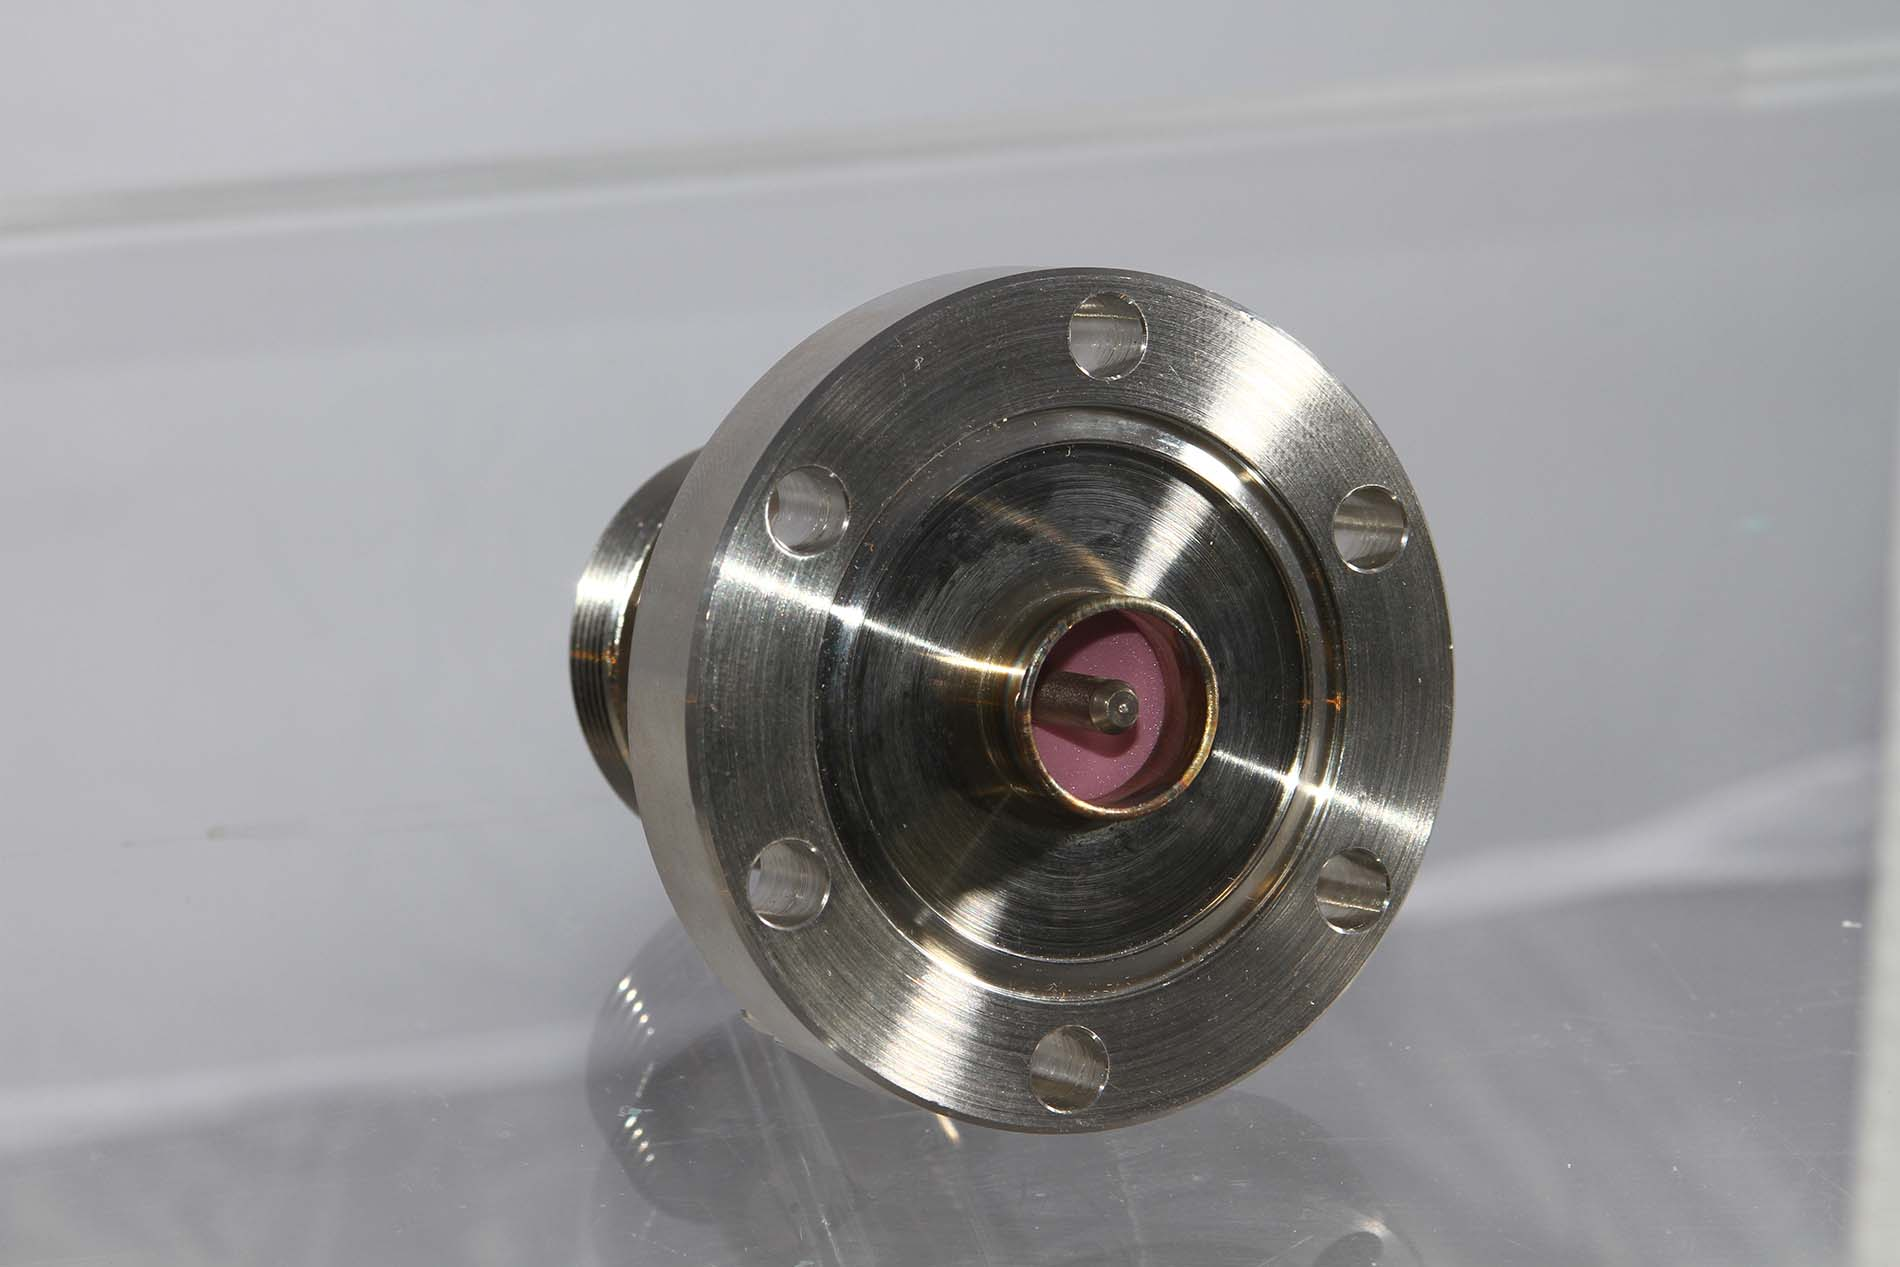
\includegraphics[width=0.33\textwidth]{../../tex/images/FID_feedthrough2}%
	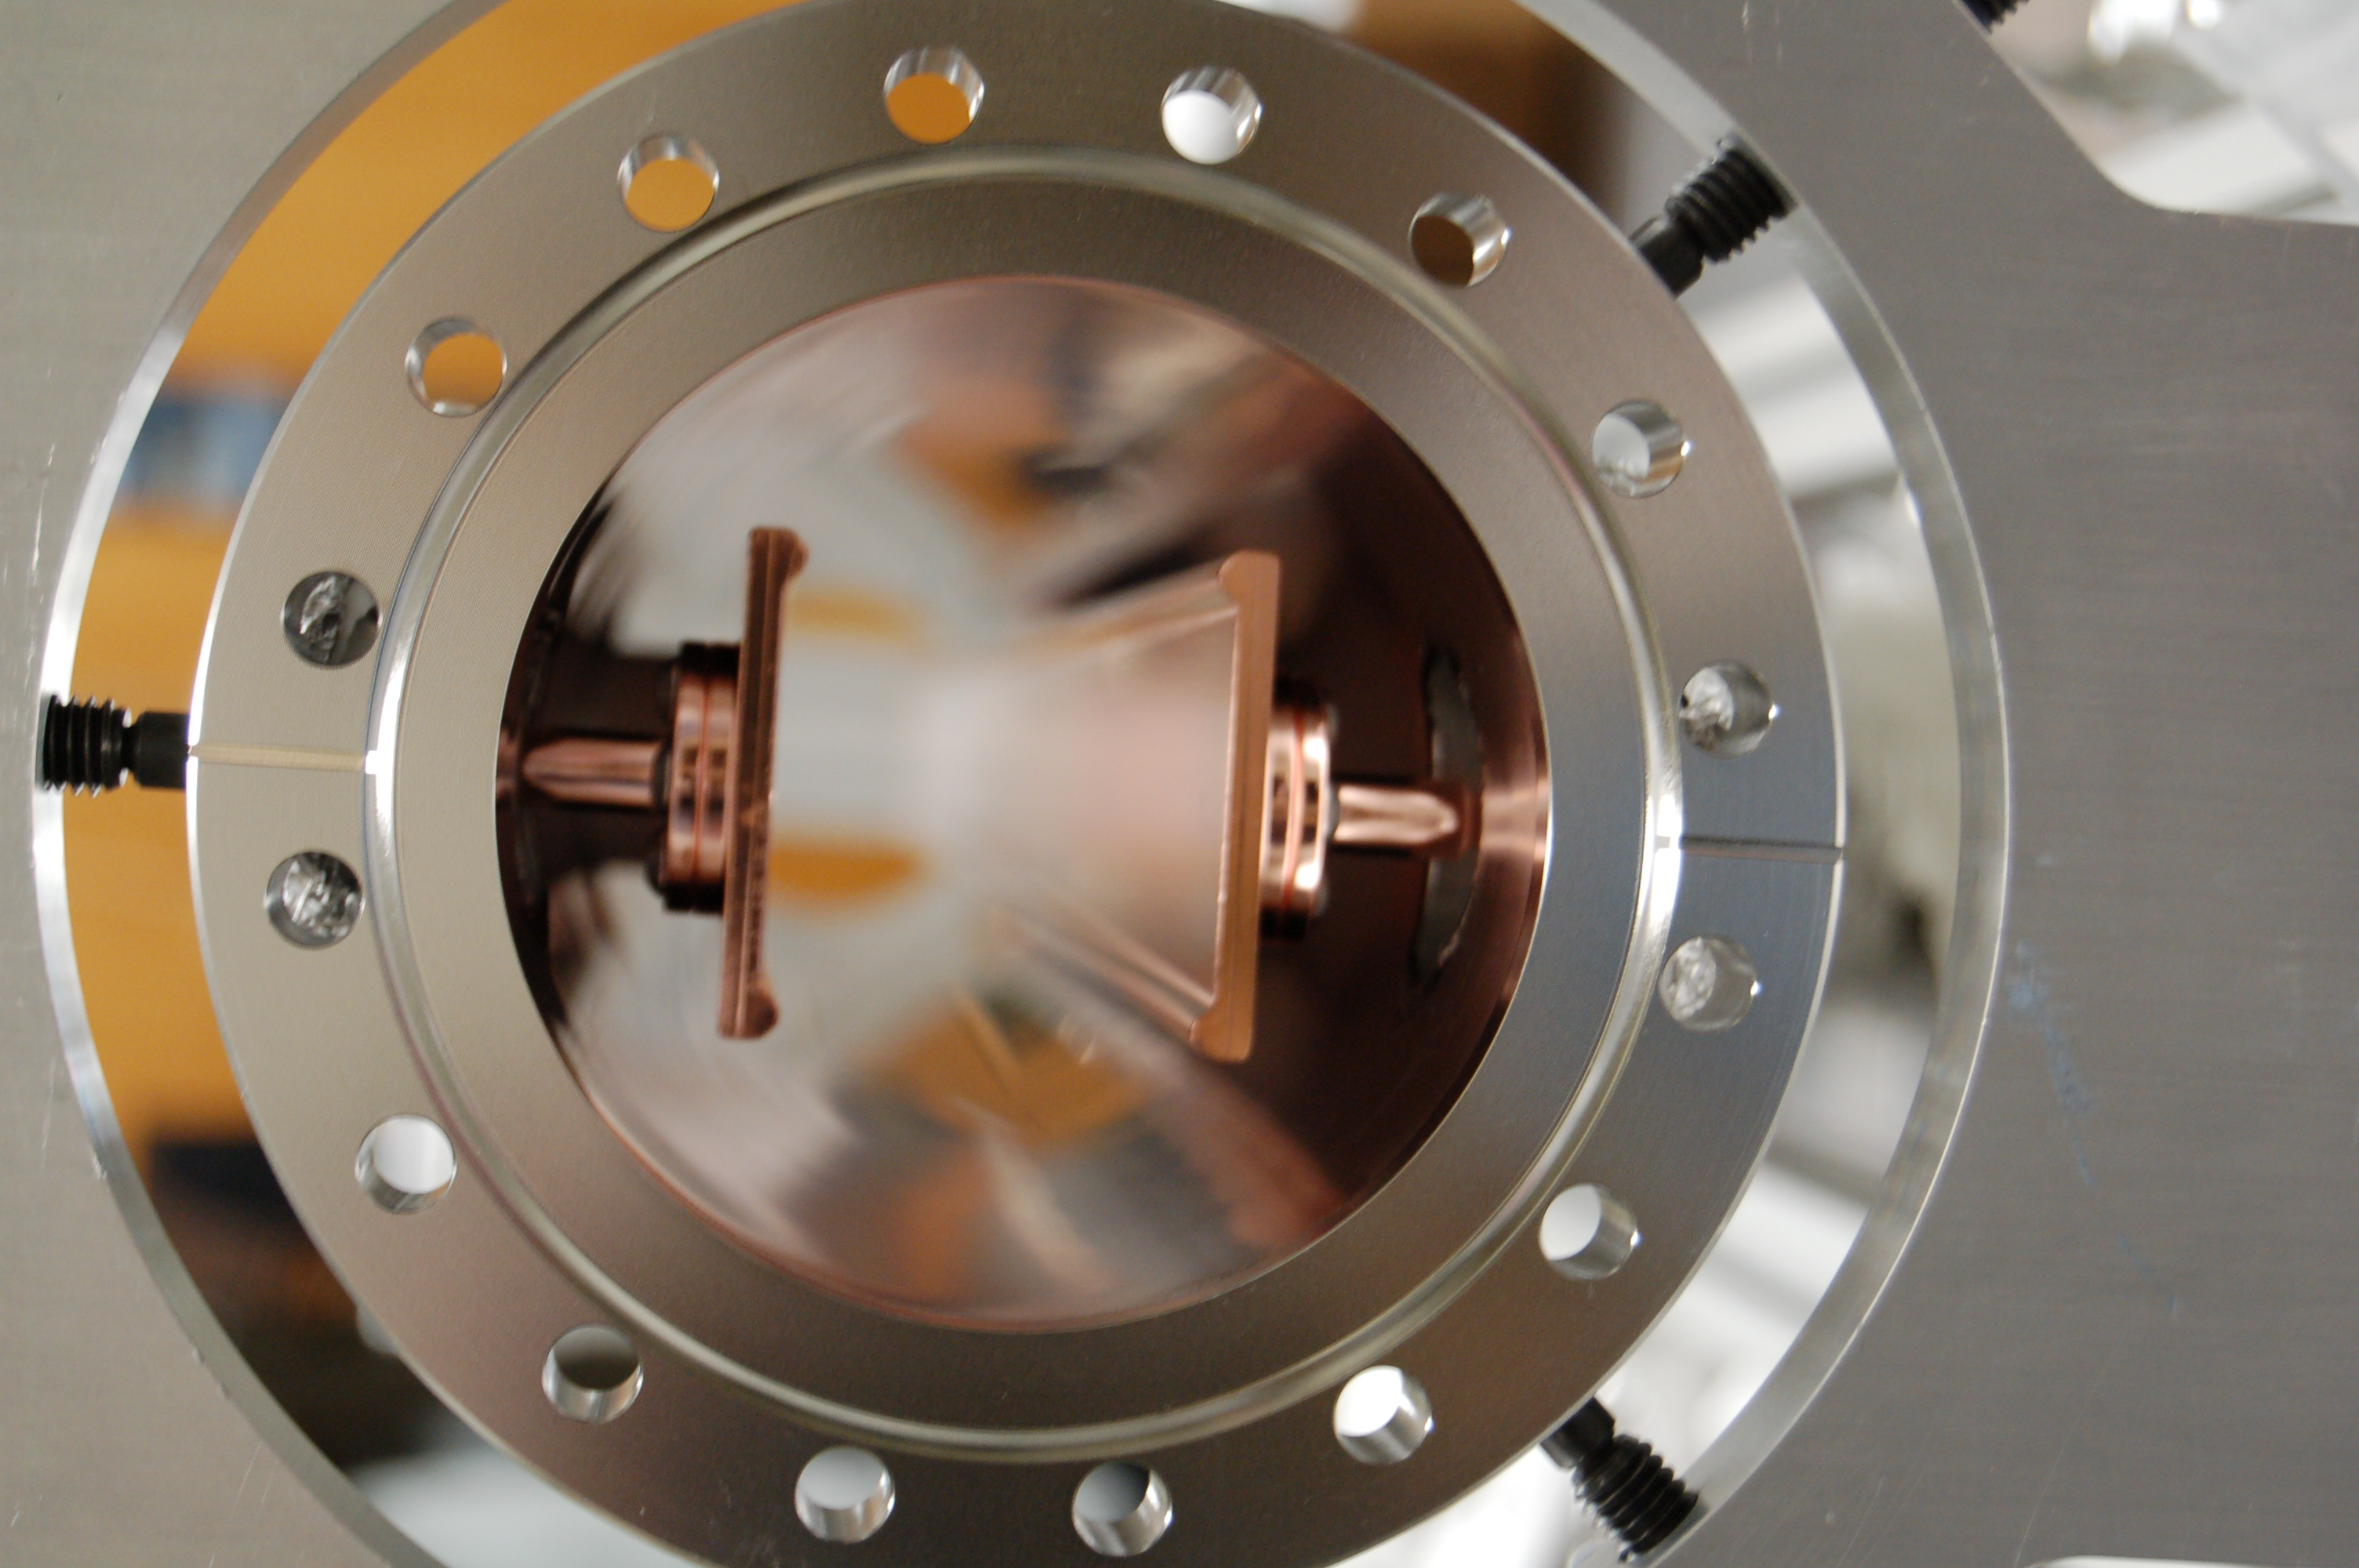
\includegraphics[width=0.33\textwidth]{../../tex/images/kicker_plates}
\end{frame}

\begin{frame}
	\frametitle{High Voltage and TDR Test}
	TDR = Time Domain Reflectometer
	\vspace{1em}
	
	\centering
	\Wider[4em]{
	\begin{minipage}{0.5\textwidth}
		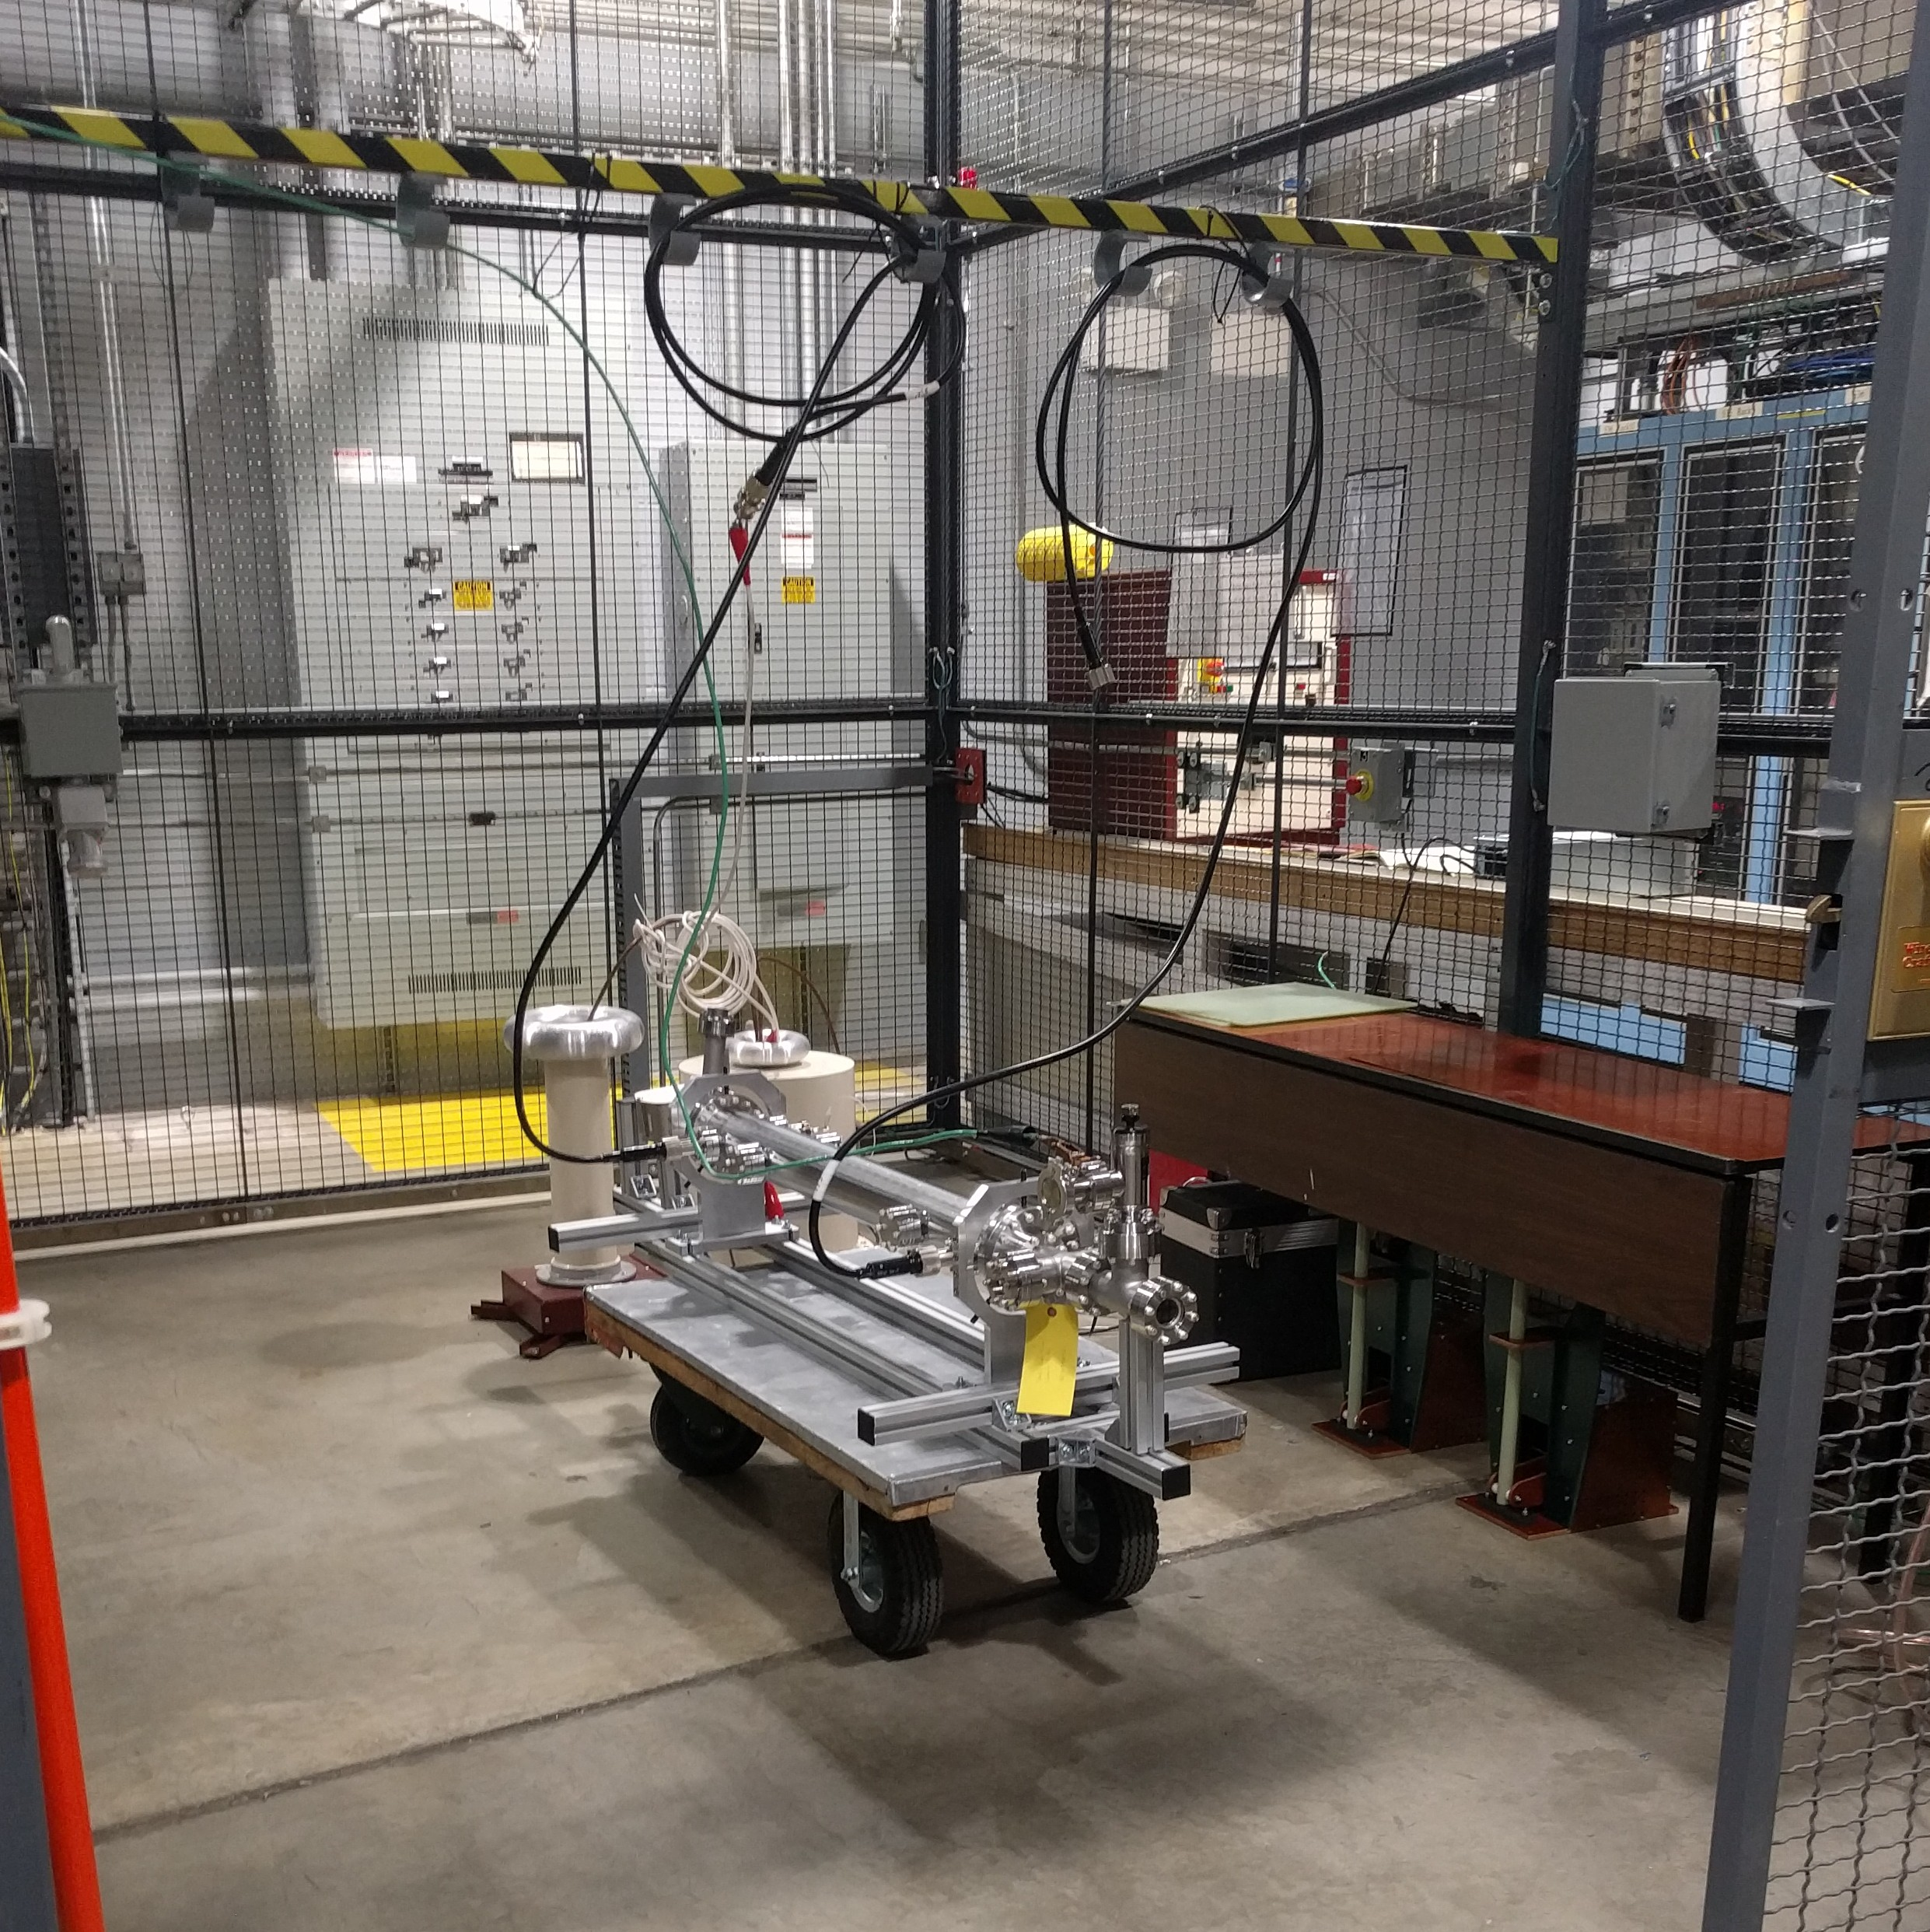
\includegraphics[width=0.9\textwidth]{../../tex/images/kicker1}
	\end{minipage}
	\hspace{1em}%
	\begin{minipage}{0.45\textwidth}
			\vspace{-2em}
		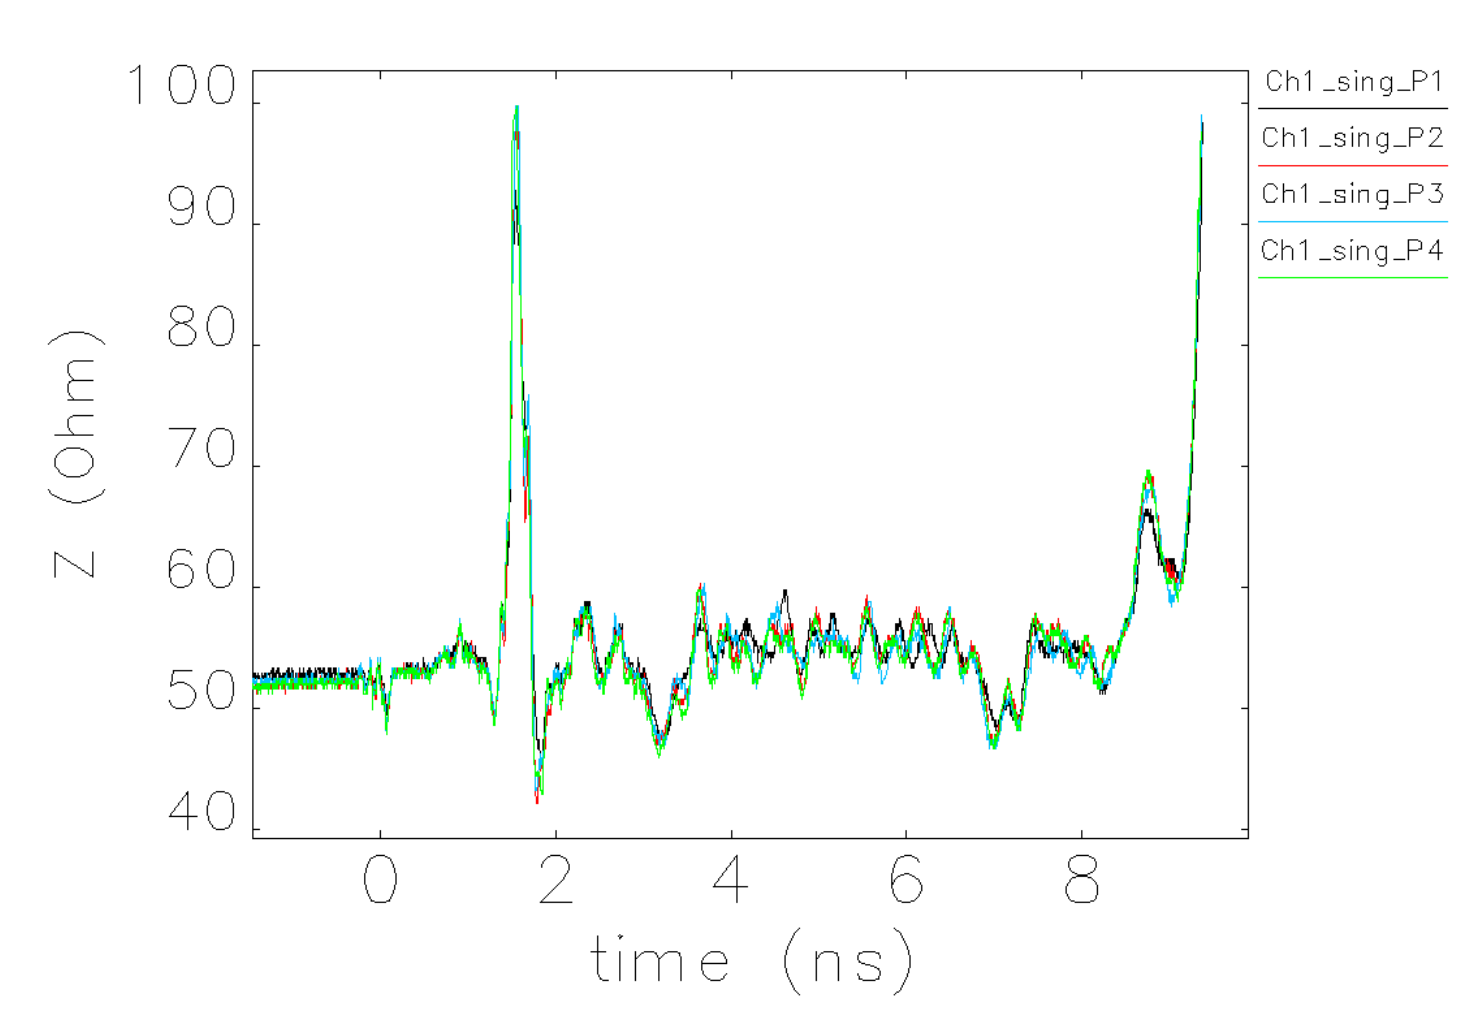
\includegraphics[width=\textwidth]{../../tex/images/TDR_AWA_kicker}
		\small *Plot courtesy of C.Y. Yao
	\end{minipage}
}	
\end{frame}

\begin{frame}
	\frametitle{Kicker YAG Screen Data}
	\begin{itemize}
		\item V = voltage supplied to kicker
		\item Kicker off at V=0
		\item Kicker on at V=$\pm$18 and V=$\pm$22
	\end{itemize}
\vspace{1em}
	\centering
	\Wider[4em]{
	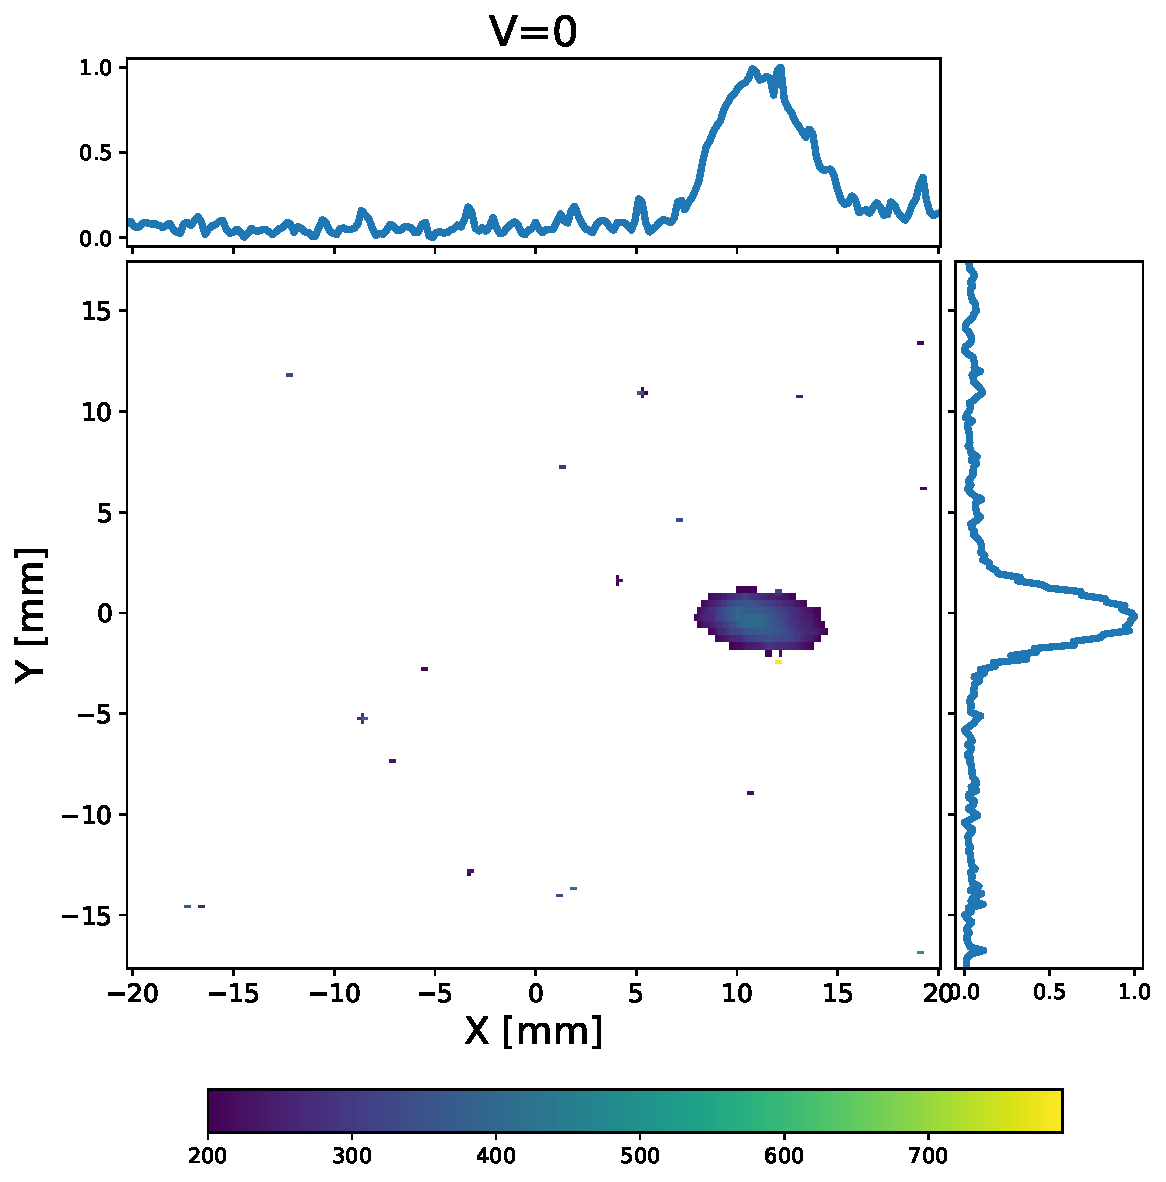
\includegraphics[width=0.33\textwidth]{../../tex/images/yag6_kicker_voltage0}%
	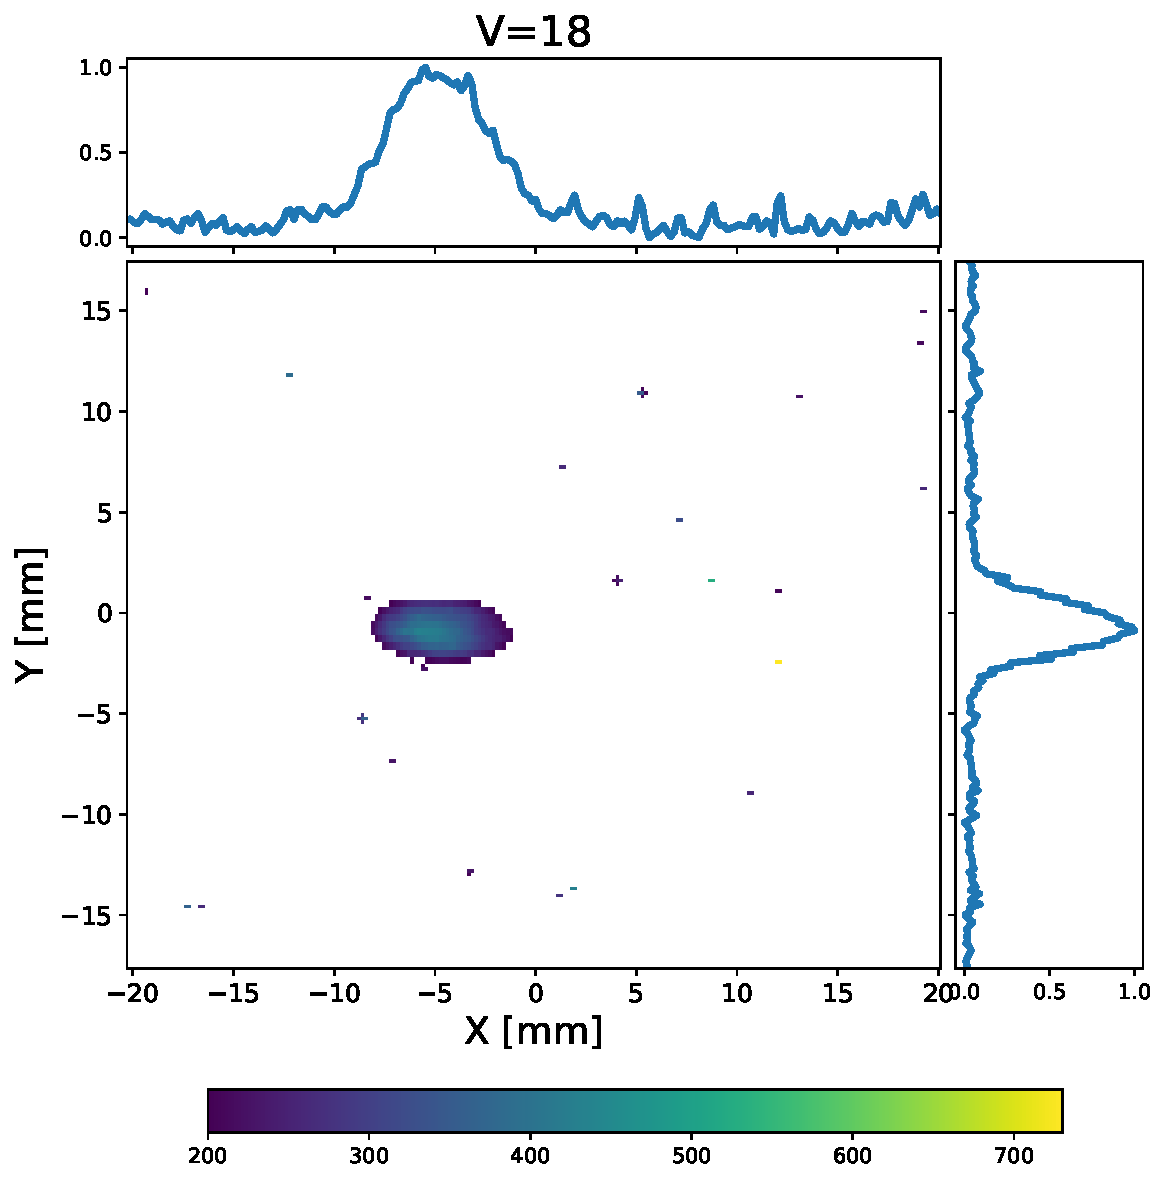
\includegraphics[width=0.33\textwidth]{../../tex/images/yag6_kicker_voltage18}%
	\includegraphics[width=0.33\textwidth]{../../tex/images/yag6_kicker_voltage22}%
}
\end{frame}

\begin{frame}
\frametitle{Kicker Beam Size and Linearity Results}
\begin{itemize}
	\item Asymmetric laser profile
	\item Asymmetry enhanced by off axis fields in cavity
	\item Angle lower than ideal, but within range needed for TBA
\end{itemize}
\vspace{1em}
\centering
\Wider[4em]{
\includegraphics[width=0.6\textwidth]{../../tex/images/xybeamsizes_high_charge_kicker_scan_angle_asymmetric}
\includegraphics[width=0.39\textwidth]{../../tex/images/kicker_angle_comparison}
}
\end{frame}

\begin{frame}
\frametitle{Summary}
\begin{itemize}
	\item Significant groundwork done for simulations and optimization at the AWA
	\item A layout was designed for fully staged TBA using these tools
	\item TBA beam line is currently being installed
	%\item Improvement of operating conditions and design of experiments through simulation and optimization work.
	%\item Have reliable/reasonable predictions that can reduce the amount of time spent on hand tuning.
\end{itemize}

\vspace{2em}
\centering
\color{blue}{\huge{Thanks for your attention!}}
\vspace{2em}

\color{black}This project and AWA are funded by:\\
\includegraphics[width=0.5\textwidth]{../../beamer/long_talk/DOE_logo_color_cmyk-eps-converted-to}
\end{frame}

\iffalse
%%%%%%%%%%%%%%%%%%%%%%%%%%%%%%%%%%%%%%%%%%%%%%%%%%%%%%%%%%%%%%%%%%%%%%%%%%%%%%%%
\section{Backup}
\begin{frame}
	\frametitle{PETS and ACC Parameters}
	Add table here
\end{frame}

\begin{frame}
\frametitle{Backup: Code Used}
\begin{itemize}
	\setlength\itemsep{2em}
	\item Used python library NLopt: \url{http://ab-initio.mit.edu/wiki/index.php/Main_Page}
	
	\item Code summary can be found at: \url{http://www.mcs.anl.gov/~jlarson/AWA}
	
	\item Complete repo at: \url{git@xgitlab.cels.anl.gov:jmlarson/emittance_minimization.git}
\end{itemize}	
\end{frame}
%%%%%%%%%%%%%%%%%%%%%%%%%%%%%%%%%%%%%%%%%%%%%%%%%%%%%%%%%%%%%%%%%%%%%%%%%%%%%%%%
\fi
\end{document}
















